\documentclass[10pt, a4paper]{article}
\usepackage[top=0.6in,bottom=1.0in,left=1.0in,right=1.0in]{geometry}
\usepackage{amsmath,amssymb}
\usepackage{graphicx,float,tikz}
\usepackage{listings}
\usepackage{tcolorbox}

\fontfamily{times}
\usepackage[colorlinks = true,
            linkcolor = black,
            urlcolor  = blue,
            citecolor = blue,
            anchorcolor = blue]{hyperref}

\begin{document}
\begin{titlepage}
	\begin{center}
		\begin{Large}
		
		\vspace*{4cm}
		\centerline{ 	
 			
\includegraphics[scale=.9]{logo.png}
		}
		\textbf{CS 4366: Senior Capstone Project \\ Dr. Sunho Lim \\ Texas Tech University \\ Project \#5 \\ Validation and Full Demo \\ EmergenSeek}
 
		\vspace{0.5cm}
		Spring 2019 Final Report 
		\linebreak
 		by \\
		\textbf{Suhas Bacchu \\ Derek Fritz \\ Kevon Manahan \\ Annie Vo \\ Simon Woldemichael}
 
		\newpage
 		\end{Large}
	\end{center}
\end{titlepage}

\vspace*{\fill}
\vspace{-2cm}
\begin{abstract}
In this final report, we describe and detail the validation of EmergenSeek, a multiuse, cross-platform mobile application providing simple access to emergency services and contact connections. As with previous reports, we will structure the report by enumerating on the frontend and backend. Dissimilarly, we will only describe necessary details in the validation of our implementations, to the extent that, any other developer with some programming background will be able to successfully implement our system's components. Only necessary details will be presented to the reader and care should be taken when reading them\footnote{Concepts such as continuous integration, continuous deployment, microservices, serverless computing, NoSQL databases, APIs, and widget-based mobile development will be discussed. These new concepts may be difficult to grasp initially, but sufficient details will be provided.}. Restatements from previous deliverable reports will be made to remind the reader of pre-defined, but important information. Also, a glossary is provided at the end of the report to define terms and jargon that may be confusing or unfamiliar for the reader. \\
\textit{Keywords:} API Gateway, CI/CD, Cloud, Dart, Flutter, Golang, Lambda, Mobile, Serverless
\end{abstract}
\vspace*{\fill}
\newpage

\tableofcontents
\newpage


\section{Introduction}
\par ~ The development of EmergenSeek has been an effective software engineering experience for our group. In this final submission, we will discuss our project by (1) restating the idea, project motivations, and our successful implementations. Then, (2) we will discuss the final state of our UML diagrams and architecture, for this Spring semester. After, (3) we will discuss the development cycle for the frontend and backend and briefly touch on the microservices architecture that we follow. 

\par ~ Next, (4) a walkthrough of the discussed development lifecycle, using only necessary details and supplementing those details with additional code comments, snippets, and screenshots. This walkthrough will allow the user to understand the structure of our application, both frontend and backend. The walkthrough will not cover \emph{everything} as the amount of content necessary for a walkthrough that assumes the reader has zero prior knowledge of the systems and concepts used in our project would take an obstructive amount of explanation. Then, (5) we will describe the current state of our serverless application repository; our collection of Lambda functions. To end (6) on our discussion of the validation, we will display Flutter views of the mobile application and their respective functionality. 

\par ~ It is very important to note that our project uses programming languages which are young in maturity and may not be familiar to the reader. But, our backend, written in Go, has syntax very similar to the C and C++ programming languages. Our frontend, written in Dart, has syntax very similar to the Java programming language. As a result of these similarities, it is permissible for the reader to assume what the code does as the syntax is, for the most part, straightforward. To conclude we will detail team member contributions, implementation issues, and steps moving forward with the project.

\subsection{Walkthrough Steps}
\par ~ The previously mentioned walkthrough will consist of the following, and be enumerated for a single Lambda function and a single Flutter application screen. This section should be referred to in the \hyperref[sec:pdl]{Project Development Lifecycle} section:
\begin{enumerate}
	\item[1.] Feature expectation. Answer the question of ``What feature do we need to implement and how do we implement it?''
	\item[2.] Lambda function: Implement the feature and its expectations around the requirements of using AWS Lambda
	\item[3.] Informal testing: Get an initial working version of the API Lambda function
	\item[4.] Formal testing: Write unit tests for the implementation
	\item[5.] Integration and Infrastructure as Code: Define the deployment
	\item[6.] Continuous Integration: Do the deployment
	\item[7.] Integrate Lambda functionality with the frontend
	\begin{itemize}
		\item[7a.] Create feature view. The view is effectively the screen that the user will interact with.
		\item[7b.] Create feature model. Define how features will be referenced by the state of the application.
		\item[7c.] Interface with Lambda function. Make calls via an HTTP client to the Lambda function
	\end{itemize}
\end{enumerate}

\par ~ As all of our project code is open-source, readers are encouraged to reference the code repositories for our project. Repositories also contain additional setup notes and details. They are located at \url{https://github.com/emergenseek/backend} and \url{https://github.com/emergenseek/Flutter-Client} for our backend and frontend code, respectively. Readers who would like more insight, or have questions are welcome to open an issue or pull request on either of these GitHub repositories.

\section{Project Overview}
\subsection{Project Definition, and Implemented Features}
\par ~ EmergenSeek is a mobile application which provides users with multiuse, centralized emergency information and notification services. This application gives friends and family members priority connections in times of emergency or crisis. Our sucessfully implemented, core feature are as follows:

\begin{enumerate}
	\item[1.] S.O.S. button emergency broadcast --- Users are able to utilize the mobile client to invoke an S.O.S. button for automated notification of contacts and emergency services. 
	\item[2.] Emergency service locator --- Users are able to utilize the mobile client to search for emergency service (hospitals, and pharmacies). Currently, searching will return results up to a fixed radius of 20 miles.
	\item[3.] Granular permission definitions for contacts --- The user is given full control over what contacts receive what level of information. This is achieved by setting alert tiers on a per-contact basis.
	\item[4.] Lock screen display of health information for emergency services --- In the case of an S.O.S. situation, the user shall have their health information displayed for the convince of first respondents.
\end{enumerate}

\par ~ Additionally, successfully implemented, quality of user-experience features are as follows. While the application is still functional without them, deploying the application for public, functional use, cannot not be possible without them.
\begin{enumerate}
	\item[1.] User registration and login --- Users are able to register for an account and track their personal information, necessary in an emergency event.
	\item[2.] Settings persistence -- Users are able to change settings within the application to fit their preference.
\end{enumerate}

\subsection{Features In-progress}
\par ~ Features which are partially implemented are as follows:
\begin{enumerate}
	\item[1.] Periodic notifications to contacts (location-based polling) --- The user shall be able to utilize the mobile client to send periodically send their location information to contacts. While the logic is in-place, we currently do not have a successful implementation of repeating the location polling.
	\item[2.] Retrieval of international emergency service numbers (ambulance, fire, and police), depending on the user's current location. Connections to the front-end have not been made yet. 
\end{enumerate}

\subsection{Future Features}
\par ~ Lastly, additional quality of user-experience features that have not been, but maybe implemented in the future are:
\begin{enumerate}
	\item[1.] More extensive error handling and reporting (via something like the Catcher, a Flutter package or Sentry.io a multi-language, multi-framework error reporting and management service)
	\item[2.] More in-depth user preferences, settings and options
	\item[3.] Alternative sign-up and log-in methods (Google, Facebook, etc.)
\end{enumerate}

\section{UML and Design Documentation}
\par ~ In this section we will discuss our completed Unified Modeling Language (UML) diagrams and design documents. Items are presented with a figure of the design unit and briefly described.

\subsection{Use-case Diagram}
\begin{figure}[H]
\begin{center}
\centerline{
	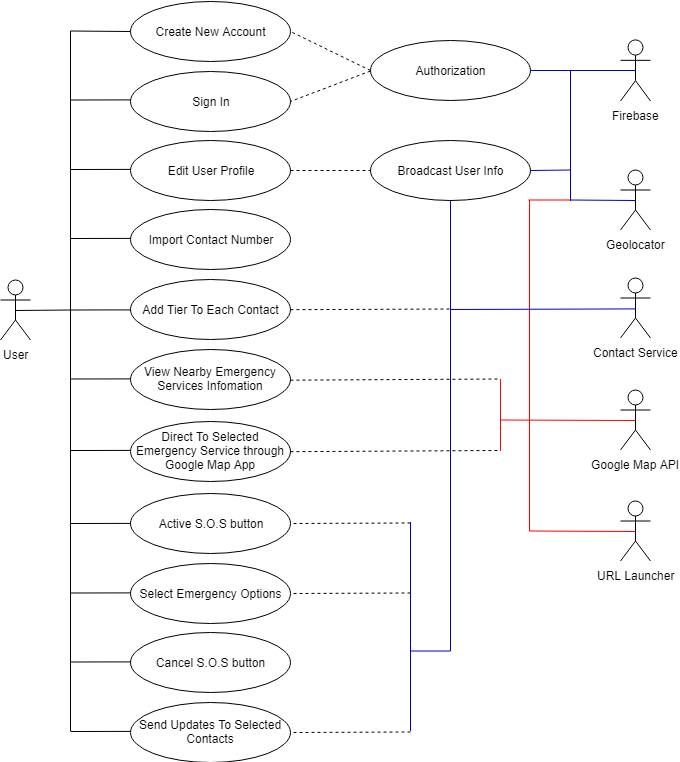
\includegraphics[scale=.6]{final-diagrams/Revised_Use_Case_Diagram.png}
}
\caption{Updated use-case diagram for the EmergenSeek application.}
\end{center}	
\end{figure}
\par ~ In this use-case diagram we detail external dependencies and their inclusion to each of the use cases. Authorization is dependent on Google's Firebase service. The broadcasting of user info is depending on using MapQuest's Geolocator API. The contact service allows us to read contacts directly from the user's phone. It is important to note that this has only been tested on Android devices. The Google Maps API coupled with the URL launcher allows us to connect our service locator with the user's native Google Maps application. Whenever the user selects a location, they will be directed to the location by tapping on the marker associated with it. Creating new accounts and signing the user in extend the authorization item. All S.O.S. button and emergency related use-cases extend the broadcasting of user info to the backend. 


\subsection{Class Diagrams}
\subsubsection{Frontend}
\par ~ For frontend class diagrams, we will first show the full models, then discuss the models, broken up into 3 smaller components, Views, Models, and Services. 
\begin{figure}[H]
\begin{center}
\centerline{
	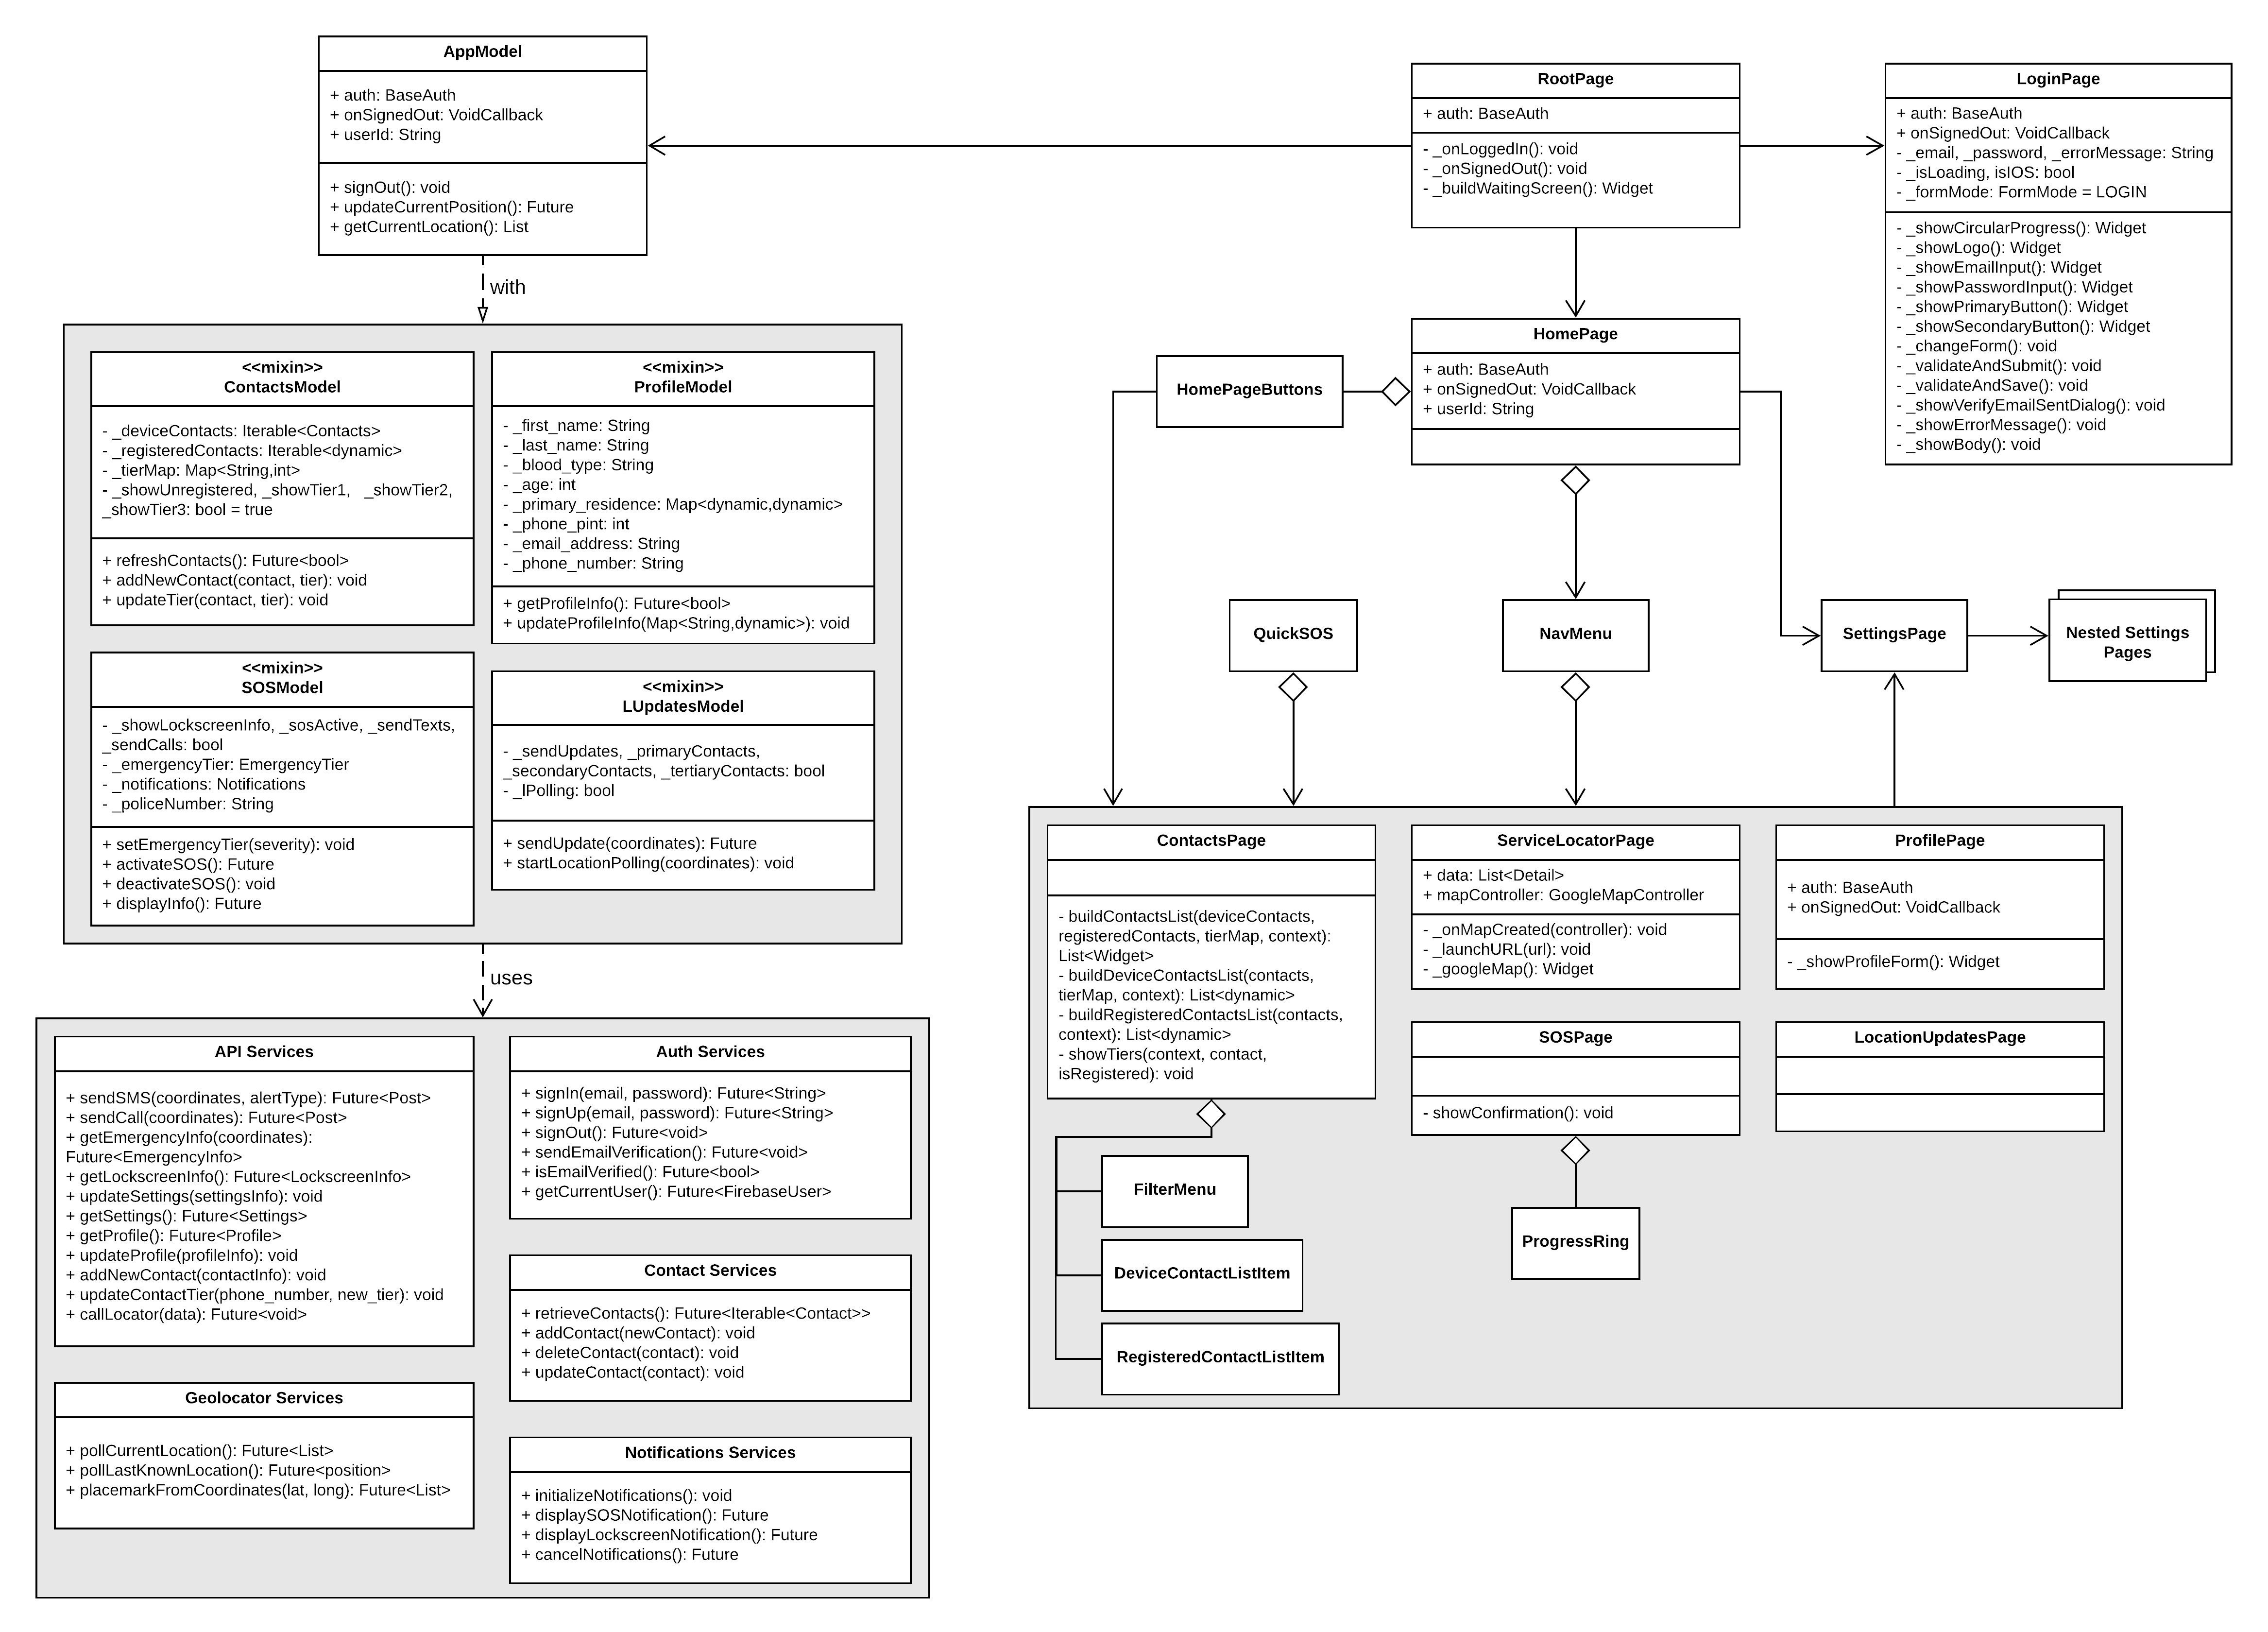
\includegraphics[scale=.13]{final-diagrams/EmergenSeek-Class-Diagram.png}
}
\caption{Full class diagram for the frontend.}
\end{center}	
\end{figure}

\begin{figure}[H]
\begin{center}
\centerline{
	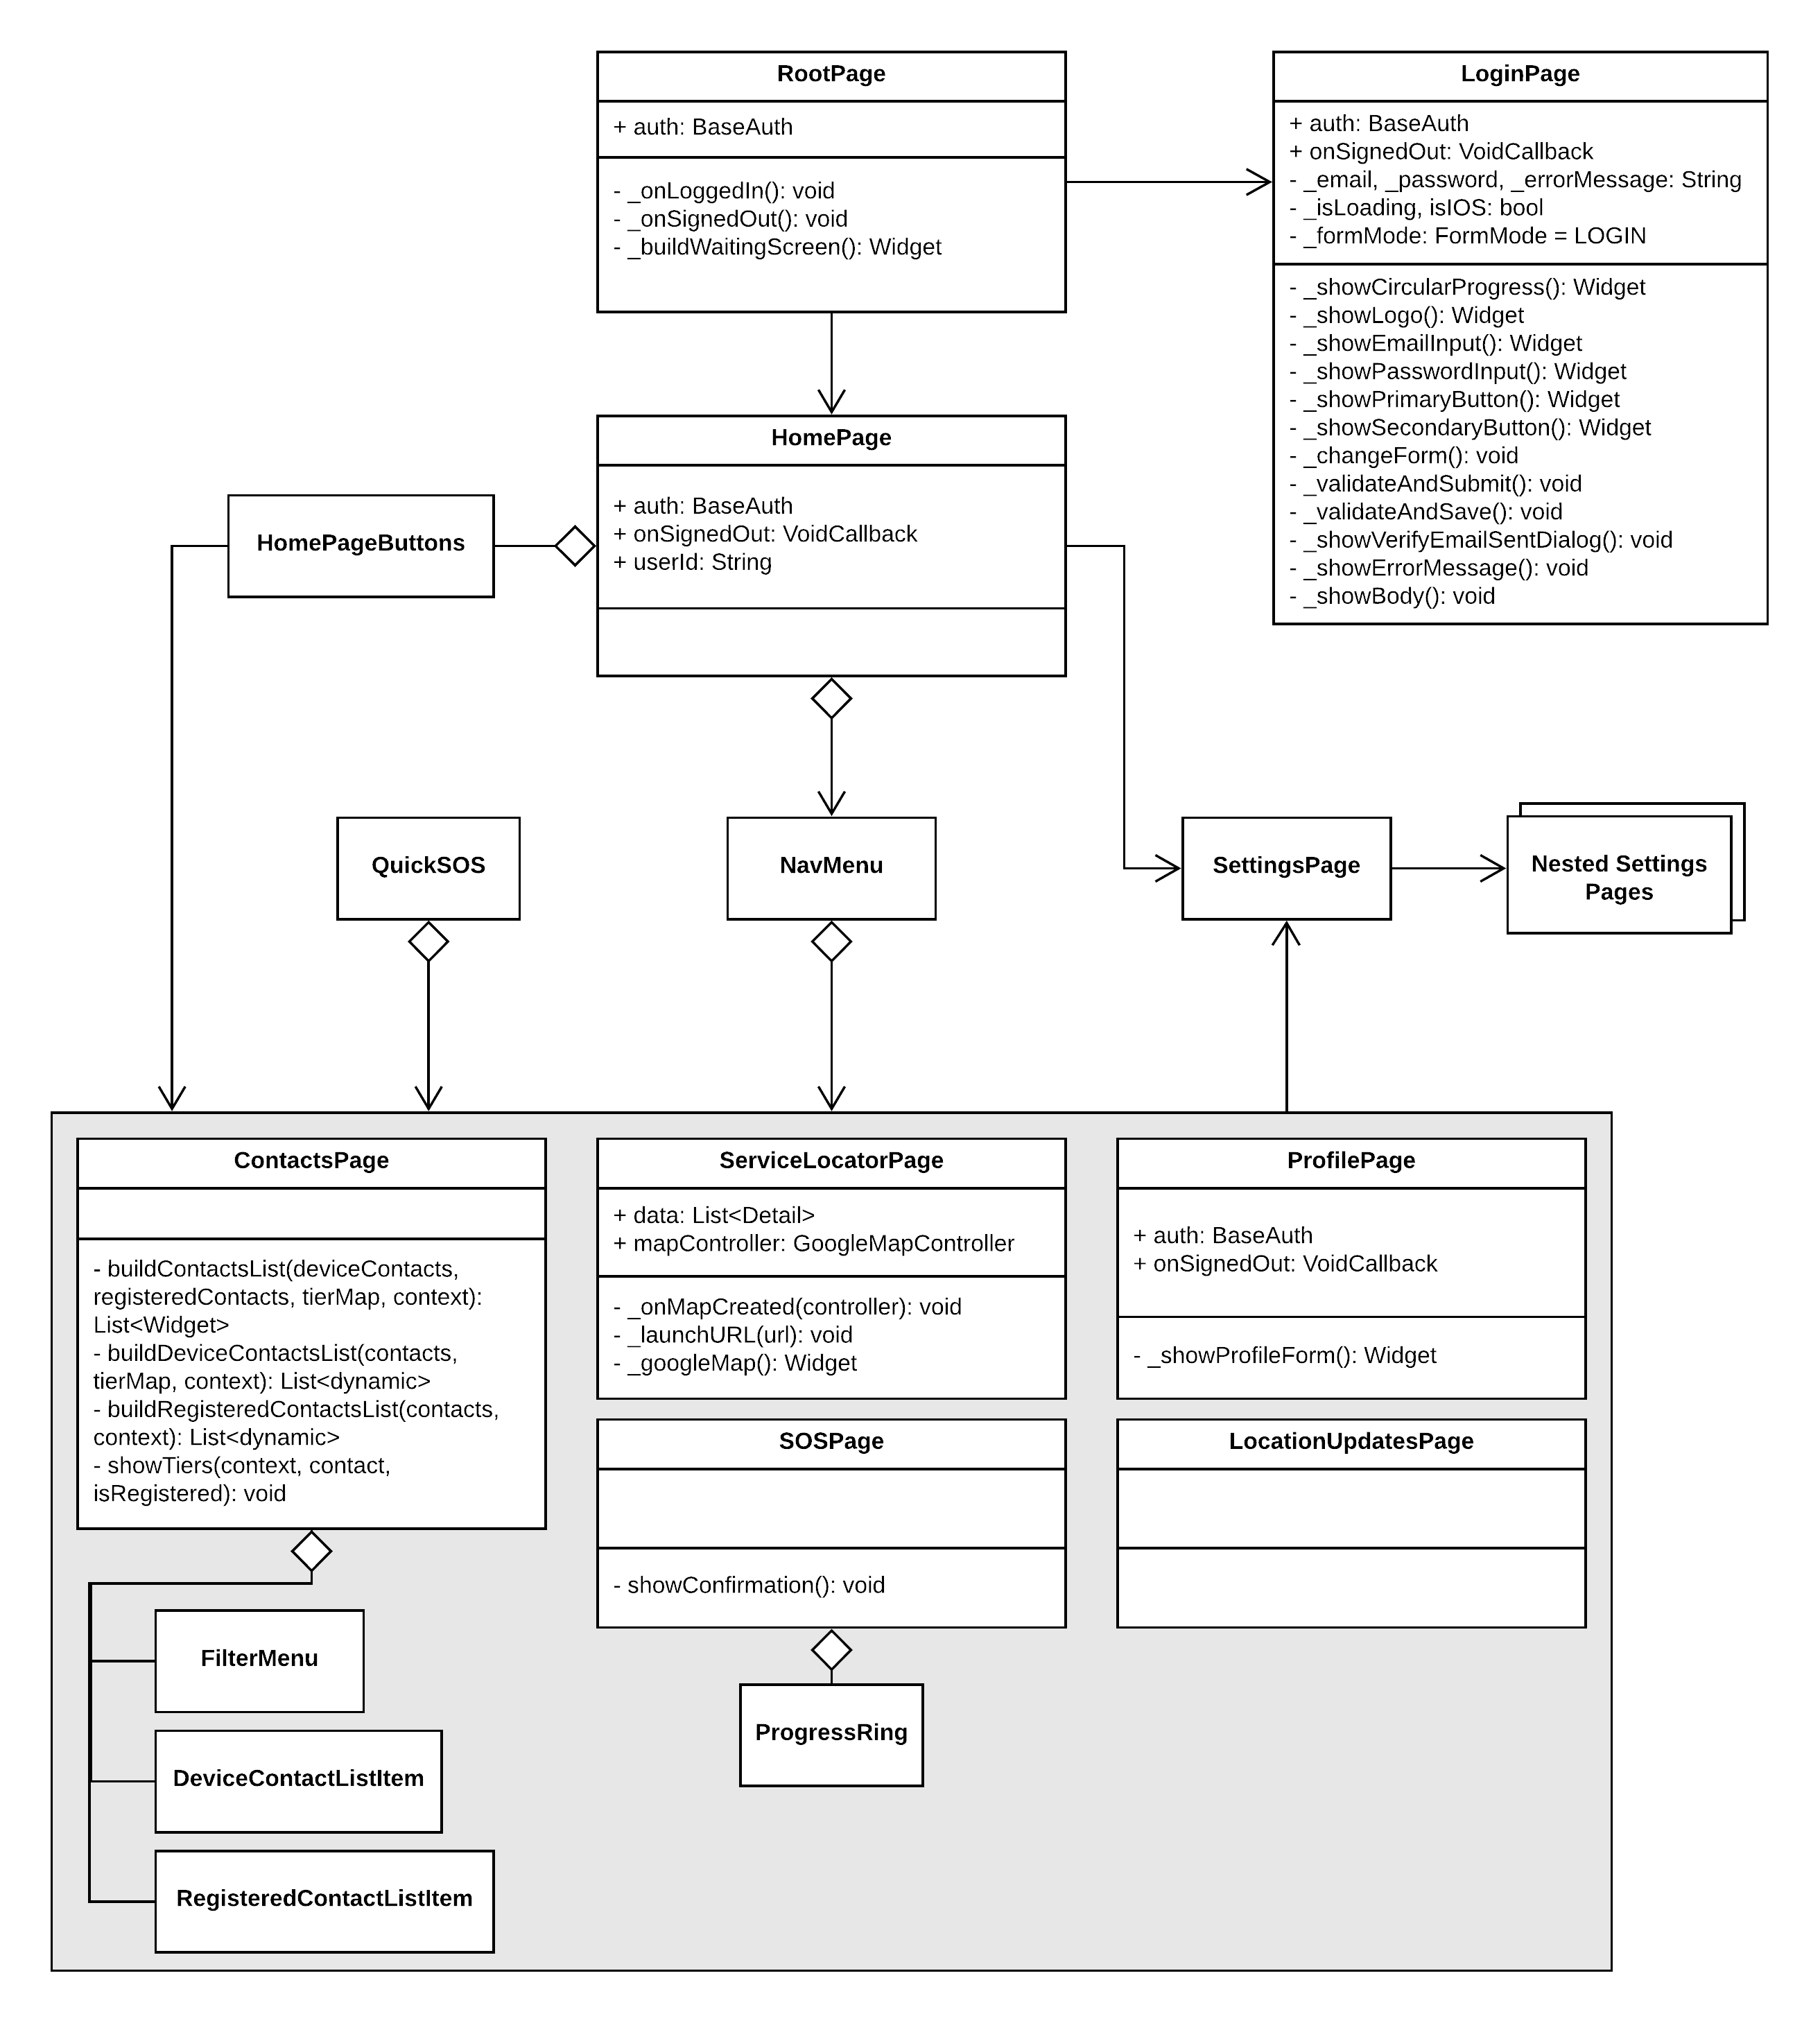
\includegraphics[scale=.23]{final-diagrams/Views-UML.png}
}
\caption{View UML class diagram for the frontend.}
\end{center}	
\end{figure}

\par ~ The application's views begins via a RootPage, this root page can be thought of a session manager keeping track of the user though an \texttt{auth} object. This object tracks actions that occur on certain events; if the user is logged in, signed out, or waiting for some communication with the backend to complete. This session state is managed via the LoginPage. From the RootPage we have a HomePage. This homepage is displayed once the base authentication, encapsulated as an attribute of the RootPage class, has received a successful response from Firebase and tells the application that the user is authorized. From the home page, we have buttons that connect the user to other views. These views, ContactsPage, ServiceLocatorPage, ProfilePage, LocationUpdatesPage, menus and navigations are displayed at the end of our report. 

\begin{figure}[H]
\begin{center}
\centerline{
	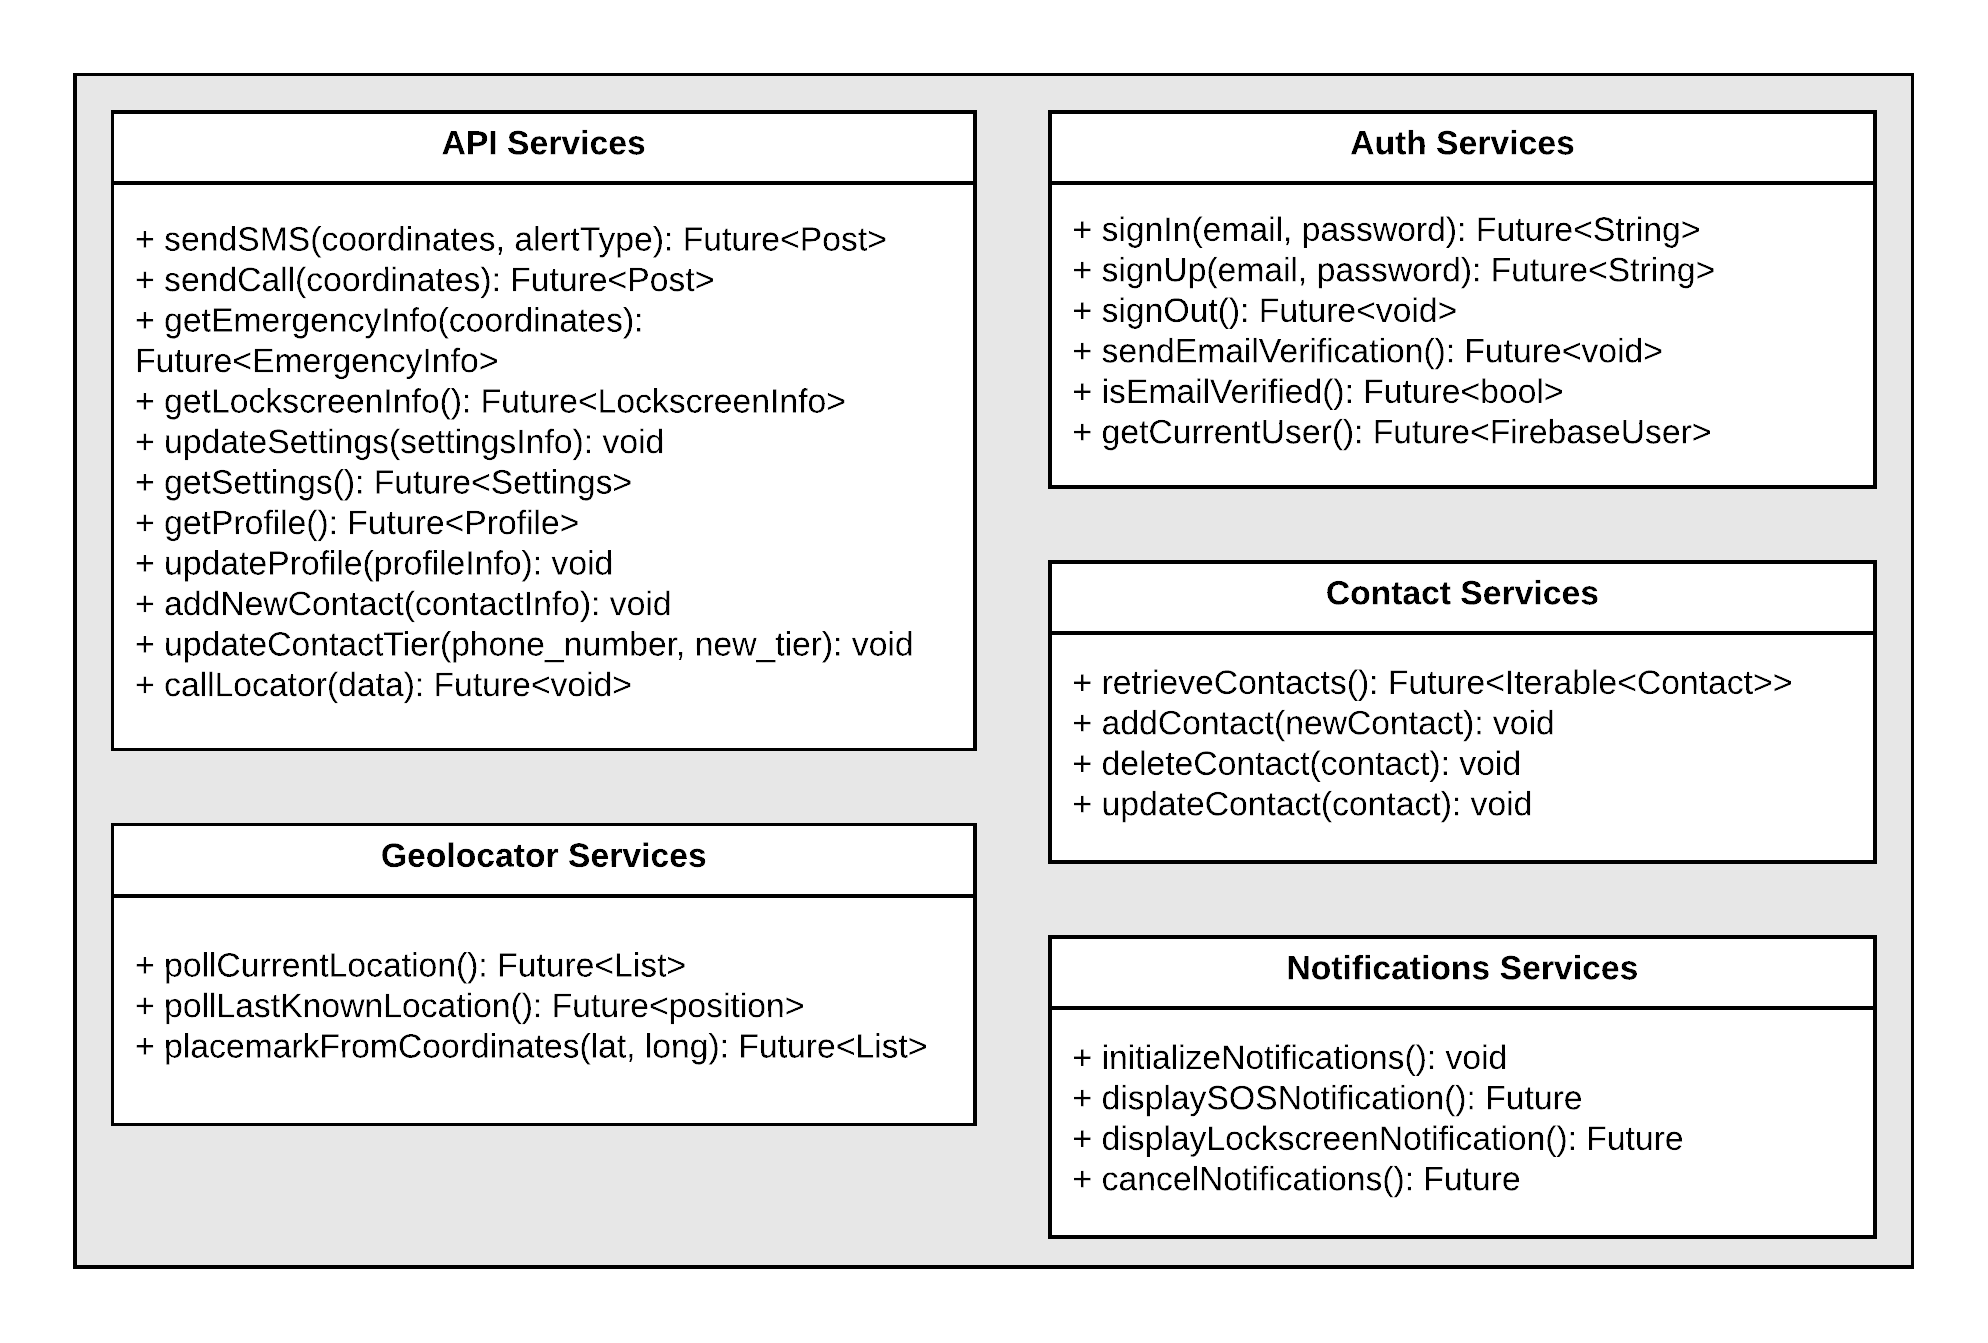
\includegraphics[scale=.23]{final-diagrams/Services-UML.png}
}
\caption{Service UML class diagram for the frontend.}
\end{center}	
\end{figure}

\par ~ The application's services are necessary for managing external API's, both Firebase and our Lambda functions. The API services class encapsulates many, general API endpoints proxied by AWS API Gateway. The Auth Services clas communicates with Firebase to register, login, and logout users. The Geolocator Services class entails methods necessary for the Google Maps integrate map we use for our service locator. The Contact Services class communicates with the native contacts API on the device's host operating system to retrieve the user's contacts. The Notifications Services class encapsulate methods necessary for displaying notifcations on the device, both within the notifications center and on the user's lock screen. \\

\begin{figure}[H]
\begin{center}
\centerline{
	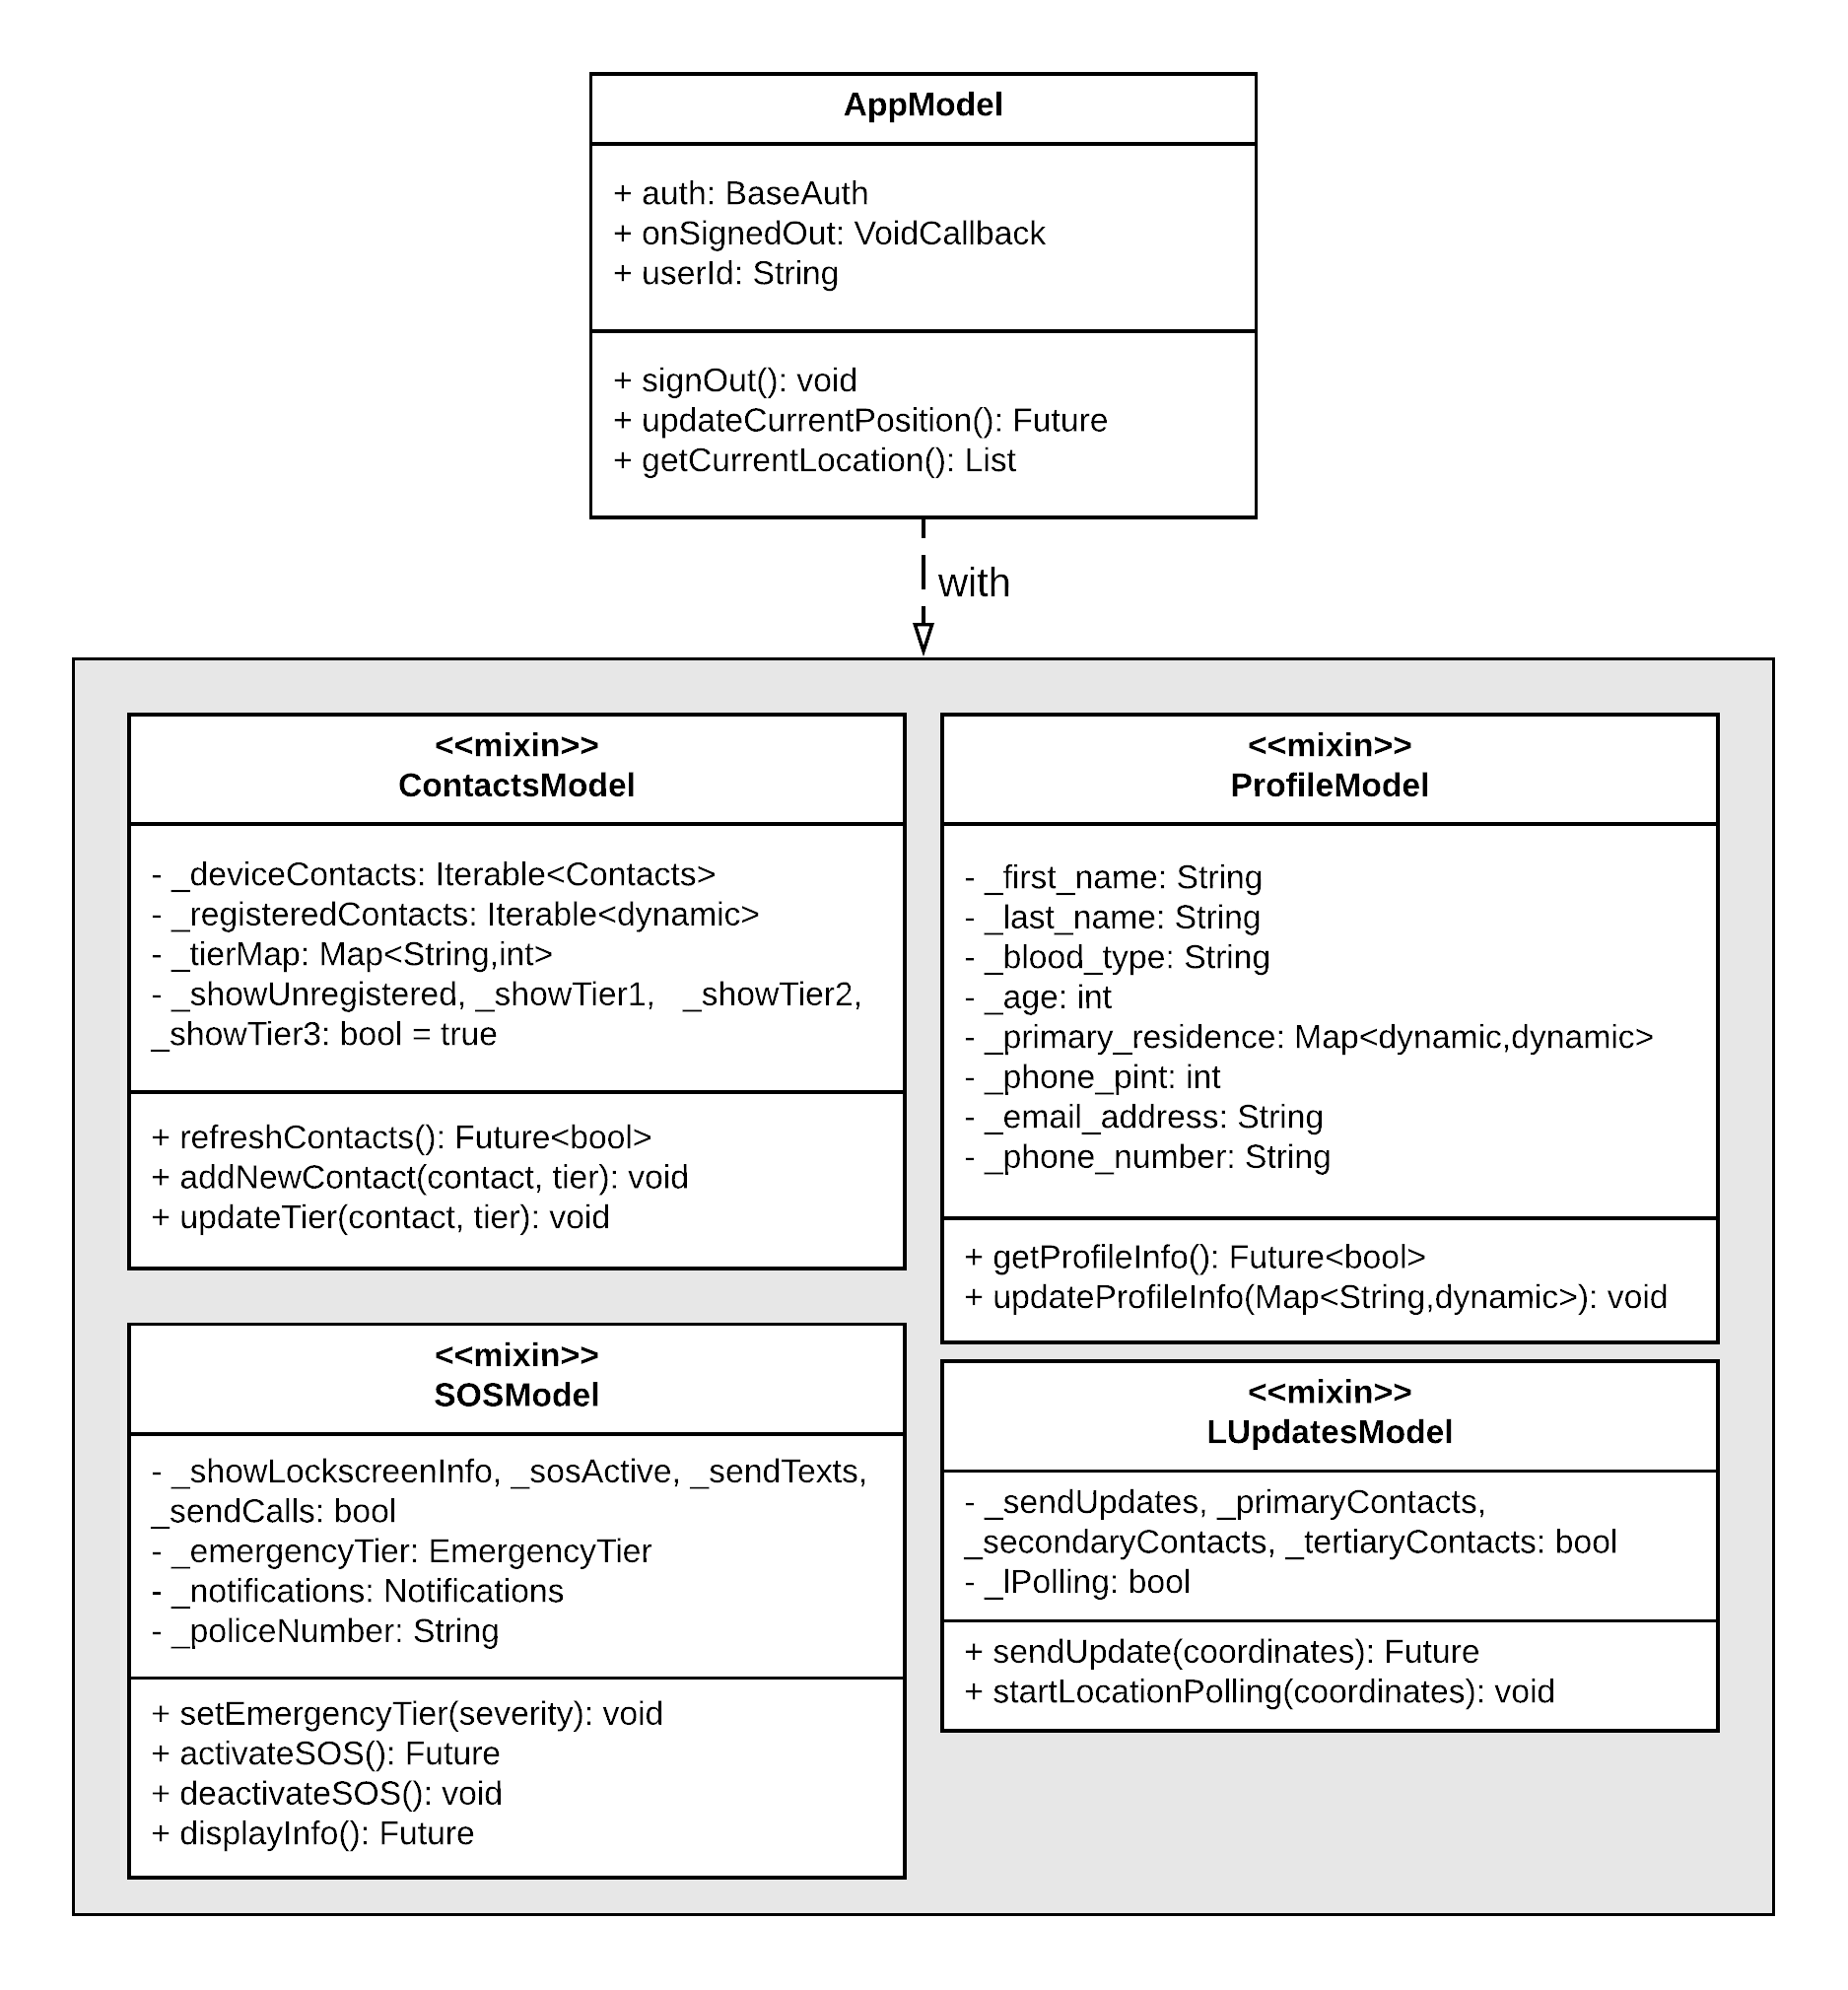
\includegraphics[scale=.37]{final-diagrams/Models-UML.png}
}
\caption{Model UML class diagram for the frontend.}
\end{center}	
\end{figure}

\par ~ The application's models and global state are tracked in an AppModel instance, this AppModel is how variables and application flow is tracked, regardless of what view the user is interacting with. The AppModel then has several \texttt{mixin} objects. A mixin, similar to inheritance, is a class which requires functionality from other base classes, but does not need to become the parent of that class. Though mixins, multiple inheritance is possible and allows our application to utilize the scoped models, discussed below.

\subsubsection{Backend}
\begin{figure}[H]
\begin{center}
\centerline{
	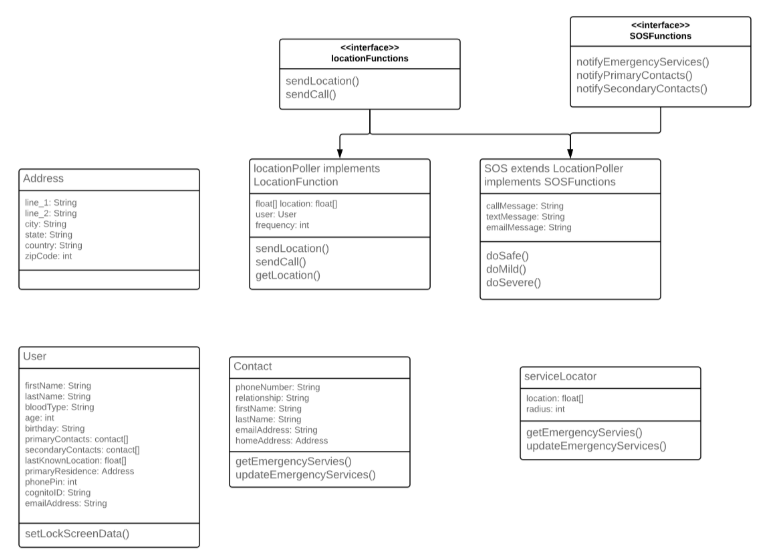
\includegraphics[scale=1.3]{final-diagrams/backend-class.PNG}
}
\caption{Class diagram for the EmergenSeek backend.}
\end{center}	
\end{figure}

\begin{figure}[H]
\begin{center}
\centerline{
	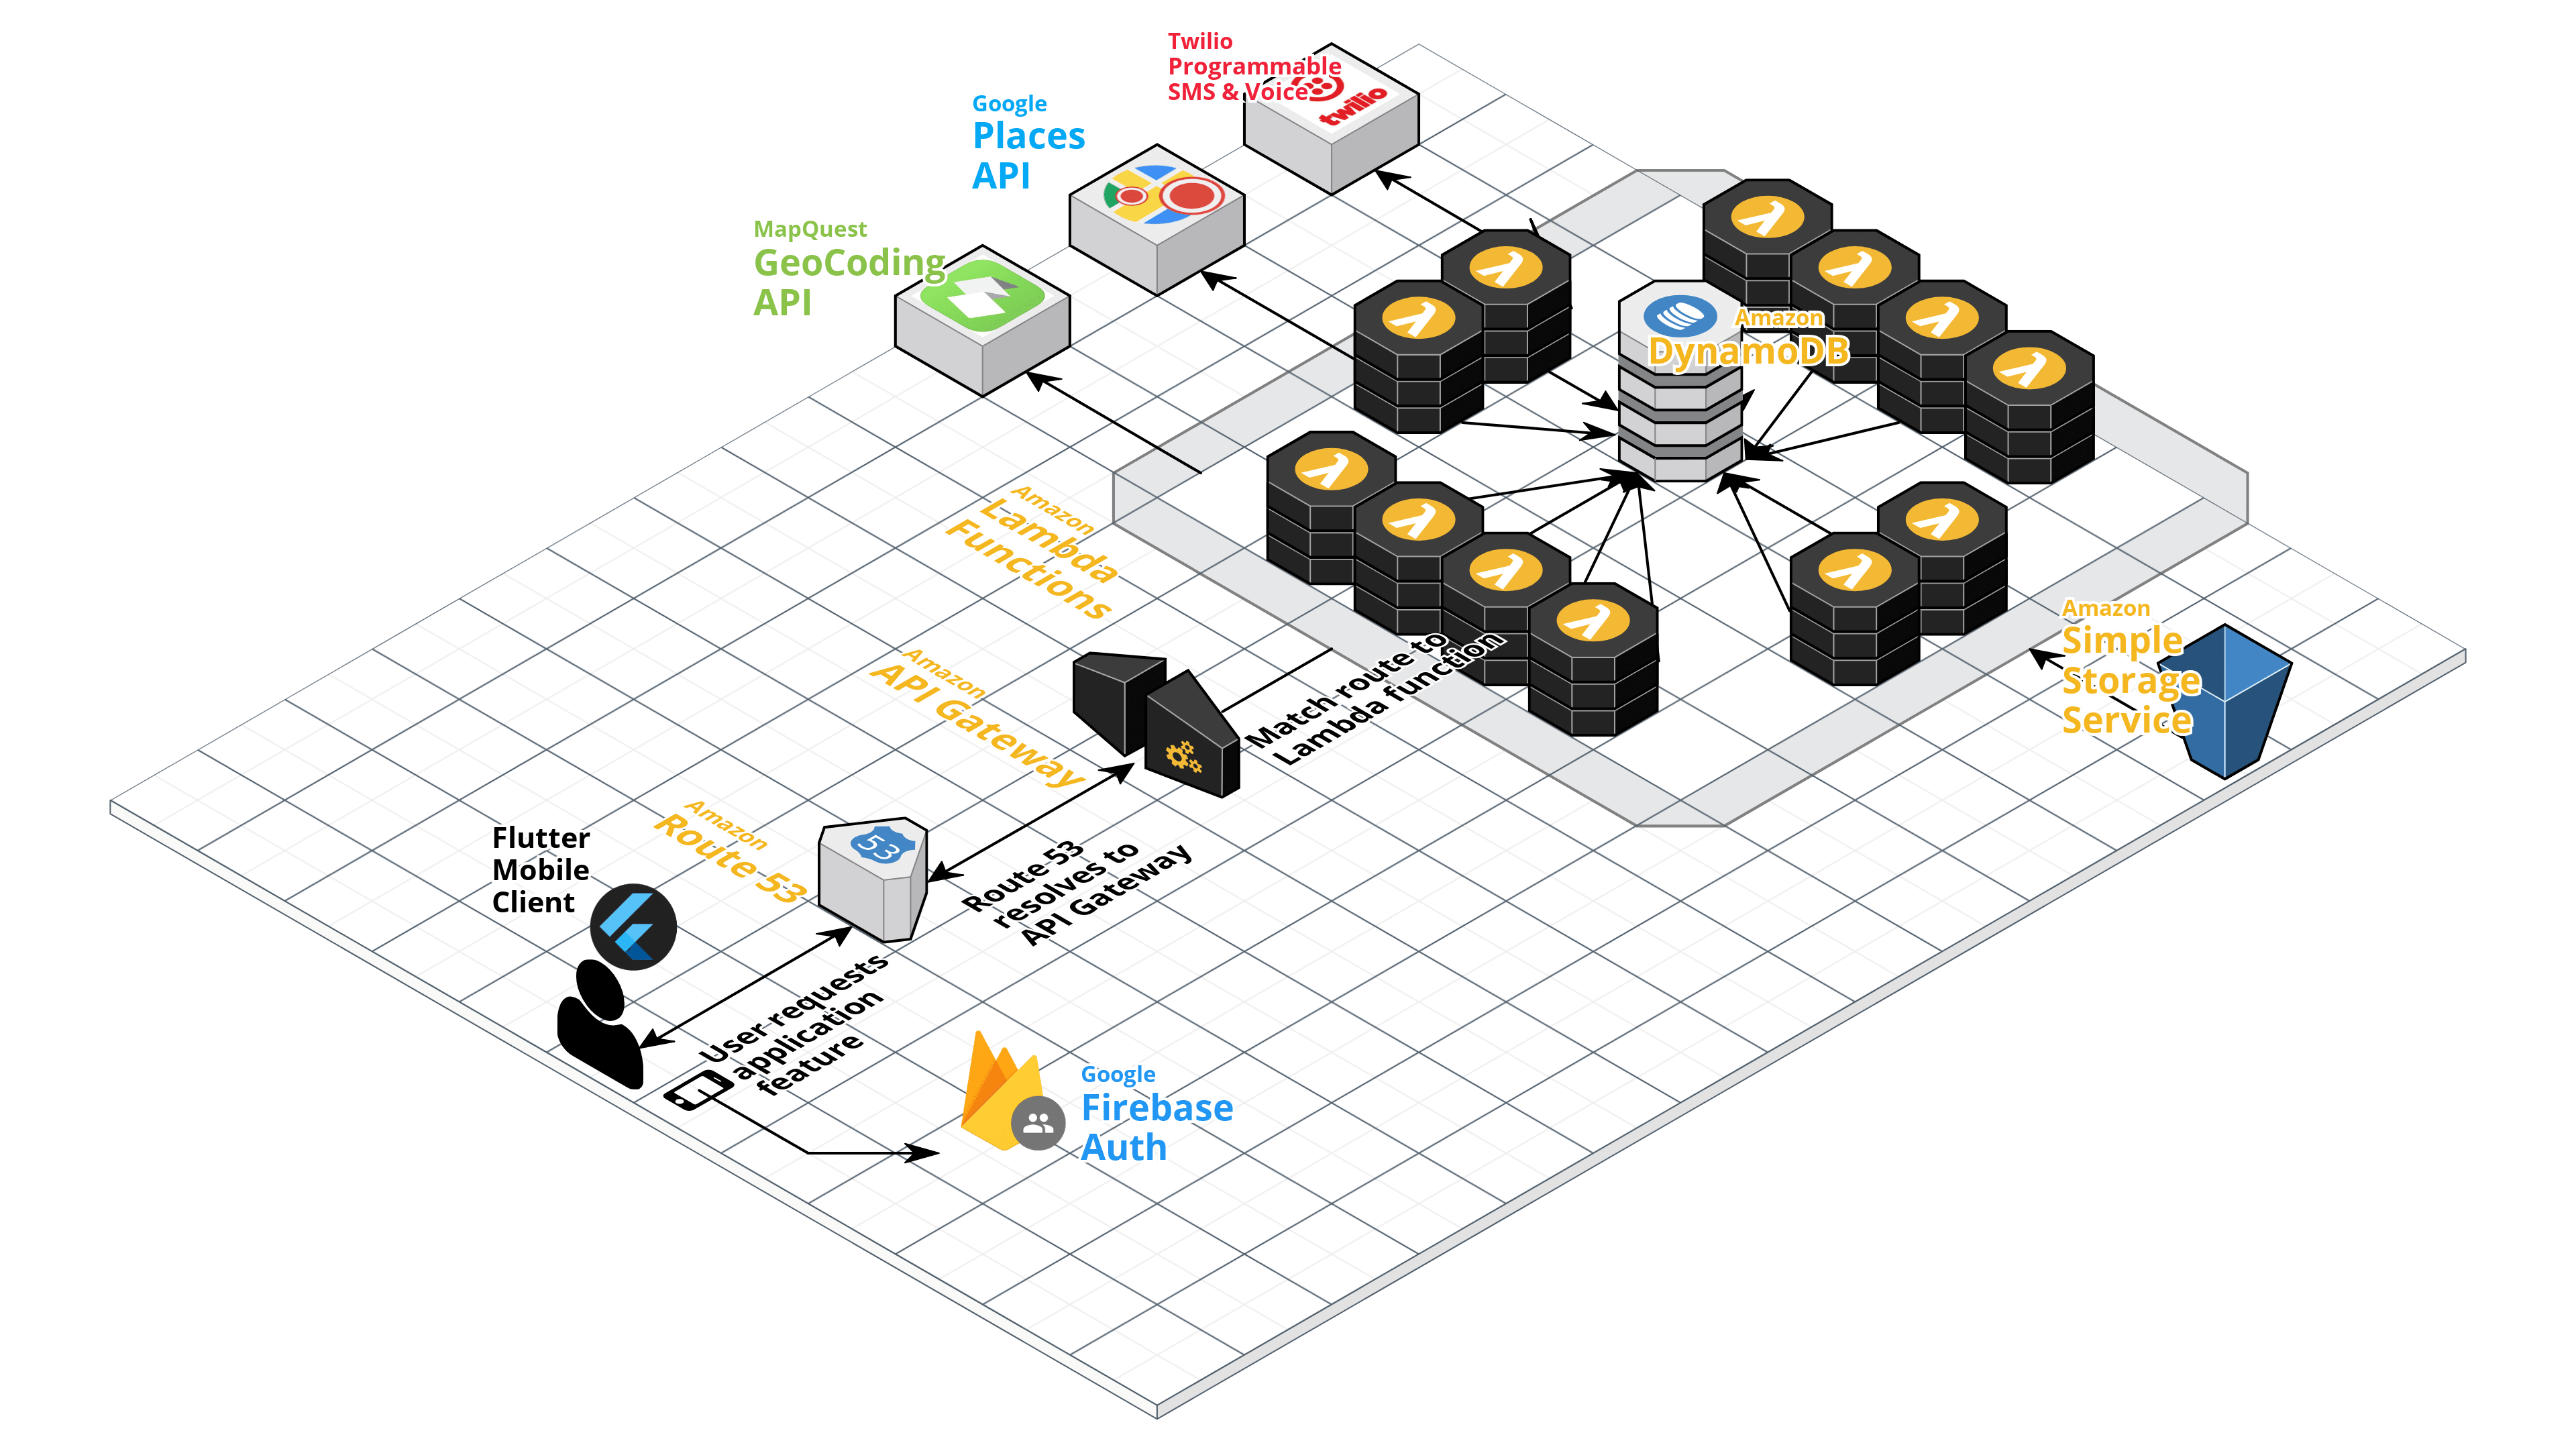
\includegraphics[scale=.2]{EmergenSeek-Backend.PNG}
}
\caption{Updated Cloudcraft diagram of the AWS resources, external APIs encapsulated by the backend, and frontend connection abstractions.}
\end{center}	
\end{figure}

\par ~ No major changes have been made to this document since previous report previsions. This class diagram should be used as a loose reference and not a literal representation of how our backend is structured for reasons related to how Go programs are written. In this class diagram for our backend we have:
\begin{enumerate}
	\item[1.] Address --- Encapsulates the data necessary for representing an address.
	\item[2.] User --- Encapsulates the data necessary for representing a user. Has 1 method which retrieves the user's information using a Lambda function for display on the lock screen.
	\item[3.] Contact --- Encapsulates the data necessary for representing a user's contact. Has 2 methods which get and update the contact on the emergency services map so that the user may see which of their contacts are nearby.
	\item[4.] ServiceLocator --- Encapsulates the data necessary for performing location based functions. Has two methods which will get and update emergency service locations for the map on the client.
	\item[5] LocationFunctions --- (Interface) This interface contains the polymorphic methods necessary for performing location related functions. This interface is implemented by the LocationPoller instance.
	\item[6.] SOSFunctions --- (Interface) This interface contains the polymorphic methods necessary for providing functionality to the S.O.S. button. This interface is implmeneted by the SOS instance.
	\item[7.] LocationPoller --- Encapsulates the data necessary for providing functionality to the location polling feature. This instance implements the LocationFunctions interface.
	\item[8.] SOS --- Encapsulates the data necessary for defining the SOS buttons functionality. This instance inherits the LocationPoller instance and implements the SOSFunctions interface. It should be noted that the \texttt{emailMessage} attribute does exist because for the scope of this clas we focused on and implemented SMS and voice notifications.
\end{enumerate}

\section{Implementation Details}
\par ~ The implementation of EmergenSeek may be broken of into two core components, Amazon Web Services' (AWS) Lambda and the cross-platform mobile development framework Flutter. These two components also have their own respective, external dependencies and services. Our Lambda functions were written using the Go programming language and the Flutter application depends on the Dart programming language. The following subsections should be read as a preface for the walkthrough of our development lifecycle. 

\subsection{Flutter Development - Frontend}
\par ~ For the implementation of a new feature within the client, several aspects must first be considered. Nearly every feature is broken down into three components: the feature view, the feature model, and the interfaces required to generate the content of the feature. During our development, we would typically begin a feature's implementation with the feature view. By beginning a feature's development with the feature view, we were able to prioritize the user-experience and develop a clearer goal of our features based on what would be most intuitive as a user. The feature view essentially consists of a widget representing a page within the app, along with any sub-widgets representing individual graphical components within the page. 

\par ~ Our top-level page widgets generally started off as stateless widgets, with certain widgets being refactored into stateful widgets as their requirements and responsibilities became better defined. This allowed us to minimize each widget's internal state management as much as possible, instead delegating state management to our feature models. After developing a general prototype of our feature's view, we would move onto implementing the feature model. While our stateful widgets manage small sets of internal state data, a more accessible and persistent state model was necessary for our service. To address this, we utilized Flutter's scoped models \cite{one}. Nearly every key feature possesses a feature model which contains important state data relevant to that feature. These models also provide an interface for managing the feature states from anywhere within the app. Once a feature model is created, it is included as a reference within our app-wide model which is passed into the widget hierarchy at the root of our application.

\par ~ After creating both the feature view and model, we would move onto considering how the feature would interface with our backend or third-party services. After determining which backend Lambda functions would be relevant to a specific feature, the respective API requests would be written as modular functions within an API service class. Some features required additional Flutter plugins to generate their content as well, which would be imported and utilized within a wrapper class. After implementing our feature services, we would then integrate the appropriate calls within the feature model. We would then add our model references within the feature view and call the various model functions for accessing and managing the feature's state data. One of our main considerations in implementing new features was ensuring a responsive user-experience. Many of our features rely on retrieving and updating data from our backend, which led to challenges in rendering our views quickly. Our solution to this was utilizing Flutter's future builder widget, which allowed us to display placeholders while our API requests were sent and the responses were received and processed.


\subsection{Lambda Development - Backend}
\par ~ Before discussing our implementation, we will give some background on why we chose to use AWS Lambda. Lambda is a serverless compute service, canonically referred to as a Functions-as-a-Service (FaaS) offering. This means that we do not need to manage any servers to deploy our code. Additionally, this manged compute is scaled up and down as necessary. If our application were to, overnight, receive thousands and thousands of users, we would be able to handle that load as a result of Lambda's auto-scaling functionality. Now that we have some background of Lambda, on to the implementation details.

\par ~ To start, we create a specialized Go function that conforms to the expectations of the Lambda software development utilities provided by Amazon. This function receives an event, which is simply an HTTP request with or without a body, and returns an event; an HTTP response with a body. The logic that occurs to process the request and return a desired response is where backend logic comes in. Though communication of various APIs (Google, MapQuest, and Twilio) and our DynamoDB database tables, we can produce these results to fulfill the requirements and expectations desired by our frontend users. These users do not have to think about how these actions occur because they are abstracted away. Instead they only need to know the expected request parameters, and the expected response results. Additionally, because our backend is, as a whole, a REST API, we can create multiple clients on multiple platforms (i.e. web in addition to mobile). While these are not entirely all of the components necessary for developing a fully functioning, long-term and highly scaleable application programming interface, they more than suffice for the scope of this course. 

\par ~ After implementing, formally, and informally testing the Lambda function on our local machines, it is ready for deployment. This deployment happens in three stages, all managed by AWS CodeStar. The first stage happens whenever a push to our \texttt{master} Git branch is done. AWS CodeStar will trigger a build via the CodeBuild service. When the build is triggered, the second stage will begin. CodeBuild will read the buildspec.yml file in the root of our repository and build binaries out of all of the Go code responsible for each function. The binaries will then be put into a Simple Storage Service bucket so that CloudFormation may retrieve them when creating each Lambda function and associating an API Gateway endpoint to it. CloudFormation is a key part of step three, the deployment. After the binaries have been build and put in an accessible place, CloudFormation will generate updates to our infrastructure by referencing a template.yml file, also in the root of our repository. This ever important, template.yml is referred to as Infrastructure as Code. This YAML definition will be enumerated on in the next section.

\vspace{2mm}
\begin{tcolorbox}
	\emph{Microservices vs. Monoliths} \\
\par ~ As students, a monolithic projects are something that we are very familiar with. A monolith is a centralized codebase that contains all of the components and assets of a project or product. Creating a monolith is definitely a lot simpler because everything relating to the project has the same locality. They typically run on the same server, use the same resources (CPU/RAM), are sometimes distributed as executable binaries. The real issues arise when changes need to be made and components need to be scaled. Developers of the monolith must wait on the components and features that \emph{their} assigned components and features are dependent upon before they may start working. Until then, they cannot begin development on a particular part of the product. This can be mitigated with additional planning and project management techniques, but is definitely a large negative that monoliths pose. Additionally, the core features of the monolith must all be written in 1 language, otherwise, additional and often convoluted implementations must be done for multiple languages to communicate with each other despite sharing the same locality. For example, running each language as a process and performing some form of interprocess communication using threads or internal web servers. Monoliths are very \underline{tightly-coupled} with many strong dependencies.

\vspace{2mm}
\hrule
\vspace{2mm}

\par ~ Microservices, on the other hand, are decentralized, independent components of a larger product that each do one thing well for the sake of the application as a whole. This is why we chose to follow this style of development. This is why we chose to follow a microservices architecture. We did not need to wait on one another to fulfill the implementation of a Lambda function. These \underline{loosely-coupled} components bring up many more challenges than a monolithic product, but their modularity and distributable attributes make them much easier and much faster to develop and deploy \cite{two}. 
\end{tcolorbox}
	

\section{Project Development Lifecycle} 
\label{sec:pdl}
\par ~ In this section we discuss our actual implementation details, beginning with the backend and moving on to the frontend. For the benefit of the reader, we will discuss our most complex Lambda function, ESSendEmergencyVoiceCall, which provides the frontend the ability to make phone calls via Twilio's API. The programming styles, and patterns used can be generalized to our other functions. Because of this, we will only cover the full lifecycle of one function in this section. Again, it is recommend that readers reference our GitHub repositories for more details and additional notes of reference: (\url{https://github.com/emergenseek/backend} and \url{https://github.com/emergenseek/Flutter-Client}). Details such as obtaining Twilio and MapQuest API keys, and configuring AWS are left up to the reader. 

\subsection{Go - Setup}
\par ~ First, we begin with our backend repository, in this repository we have 2 key folders, \texttt{common} and \texttt{functions}. Common encapsulates, four packages, \texttt{package database}, \texttt{package driver}, \texttt{package models}, and \texttt{package notification}. The names of these packages are self explanatory. Database encapsulates database functions, driver encapsulates important backend logic functions, models encapsulates data models, and notification encapsulates functions related to Twilio Voice and SMS communication. The const.go file defines constants used through the application and belongs to the parent package, \texttt{package common}. The functions folder encapsulates our serverless application repository, for this walk through we will only focus on ESSendEmergencyVoiceCall. Within the ESSendEmergencyVoiceCall we have 6 key files. 
\begin{enumerate}
	\item[1.] event.json -- A test request sent to the function
	\item[2.] main\_test.go -- Unit tests for the function
	\item[3.] main.go -- The function definition (Lambda handler)
	\item[4.] Makefile -- For convince, to make local testing easier
	\item[5.] request.go -- Defines the expected request body or parameters which will be sent to the function. 
	\item[6.] template.yaml -- Used for local testing of Lambda and API Gateway using the Serverless Application Model command-line interface and Docker
\end{enumerate}

\begin{figure}[H]
\minipage{0.32\textwidth}
  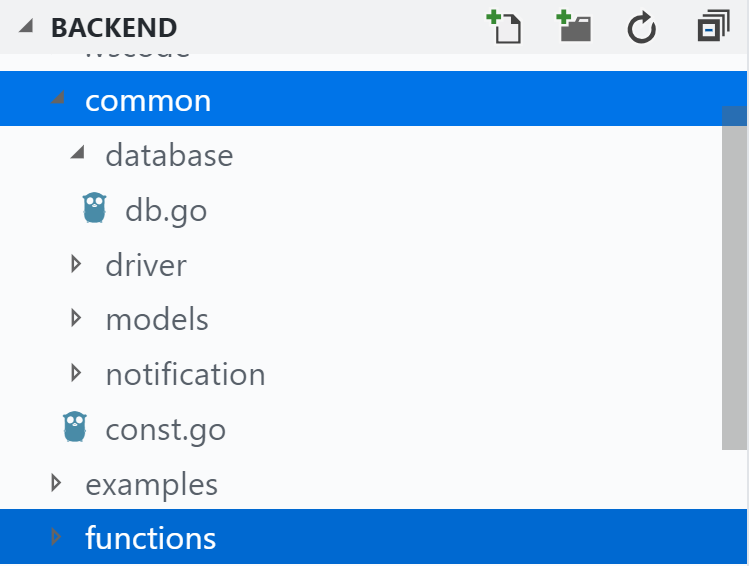
\includegraphics[width=\linewidth]{code-screenshots/one.png}
  \caption{Screenshot of the functions folder and the contents of the common folder in the backend repository.}
\endminipage\hfill
\minipage{0.32\textwidth}
  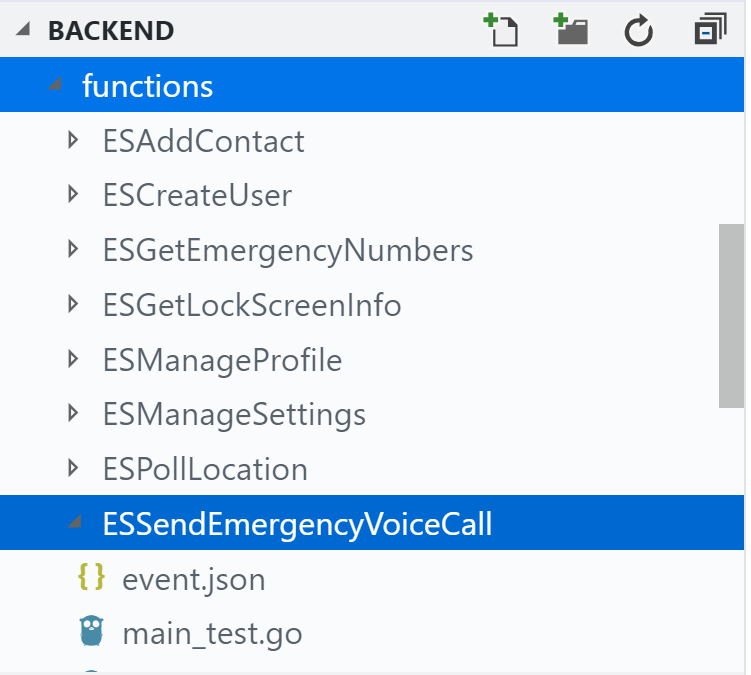
\includegraphics[width=\linewidth]{code-screenshots/two.png}
  \caption{Screenshot of the contents of the functions folder in the backend repository.}
\endminipage\hfill
\minipage{0.32\textwidth}%
  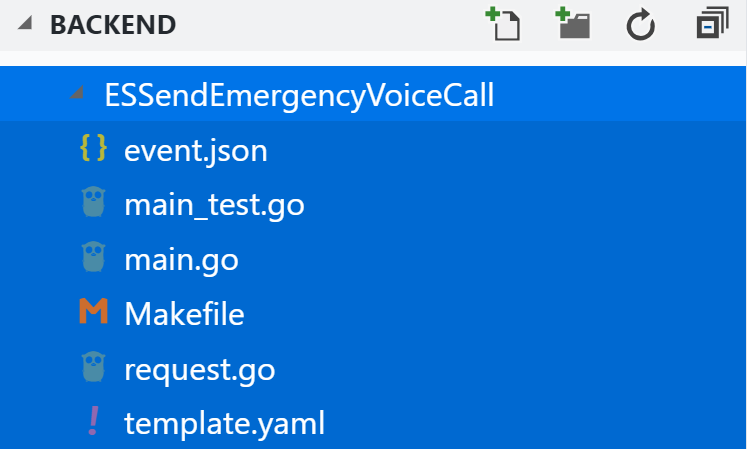
\includegraphics[width=\linewidth]{code-screenshots/three.png}
  \caption{Screenshot of the contents of the ESSendEmergencyVoiceCall repository within the functions folder.}
\endminipage
\end{figure}

\par ~ We will begin with main.go. main.go defined within the \texttt{package main} namespace, houses the \texttt{func main} function. This is a requirement of the Go programming language, the entrypoint should be called \texttt{func main} and must exist within \texttt{package main}. Within \texttt{func main} was have a call to lambda.Start and pass in Handler. Start is a function within the lambda package exposed by the "github.com/aws/aws-lambda-go/lambda" import and Handler is a function defined above func main. Anytime the ESSendEmergencyVoiceCall function is called, the code within the Handler is executed. The function passed to \texttt{lambda.Start} does not need to be called Lambda, it must simply be a function with has the expected signature; 1 input parameter of type \texttt{events.APIGatewayProxyRequest} and two return parameters of type \texttt{events.APIGatewayProxyResponse} and \texttt{error}, in that exact order.

\par ~ As we see in the screenshot, the first duty of the Handler is to verify the request. This mean to match the expectation of the API against the request body provided by the user. To do this, we use a helper function that we defined, called \texttt{verifyRequest}. If any expectations are failed, we return an error to the user. 

\begin{figure}[H]
\minipage{0.32\textwidth}
  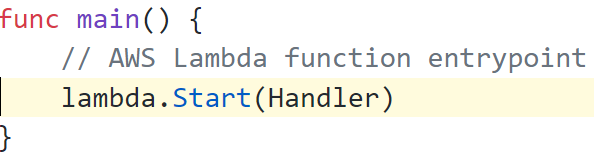
\includegraphics[width=\linewidth]{code-screenshots/four.png}
  \caption{Screenshot of \texttt{func main} within \texttt{package main}}
\endminipage\hfill
\minipage{0.6\textwidth}
  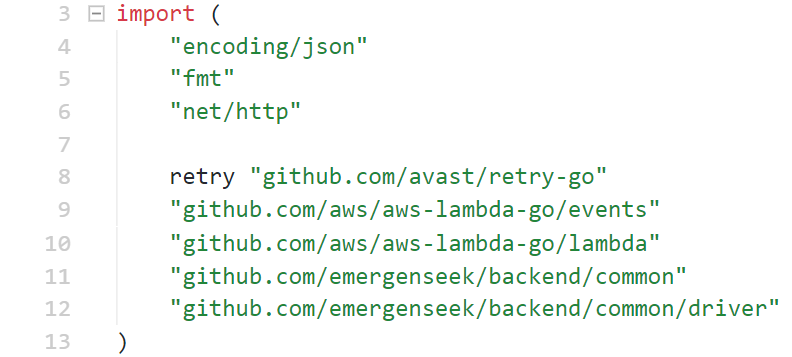
\includegraphics[width=\linewidth]{code-screenshots/seven.png}
  \caption{Screenshot of imports defined for the function. Their accessors are either defined as an alias to the left of the import name (like retry), or as the package name defined by the dependency. Standard library packages are defined above external, third-party dependencies.}
\endminipage\hfill
\end{figure}

\begin{figure}[H]
  \ 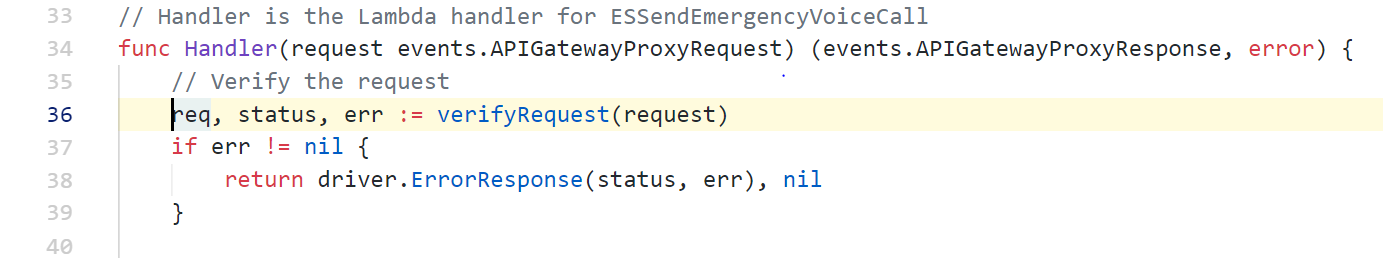
\includegraphics[scale=.6]{code-screenshots/five.png}
  \caption{Screenshot of the first few lines of the Handler definition}
\end{figure}

\begin{figure}[H]
  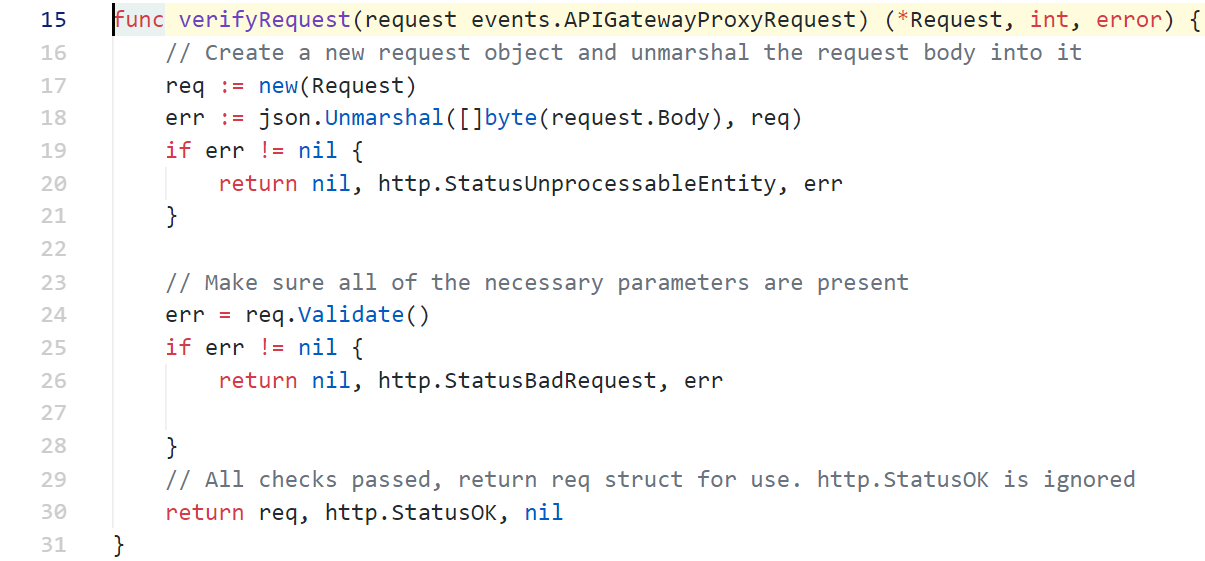
\includegraphics[scale=.6]{code-screenshots/six.png}
  \caption{Screenshot of the definition for \texttt{verifyRequest}}\label{fig:vr}
\end{figure}

\par ~ The request checked against in Figure ~\ref{fig:vr}, line 17, is defined in request.go. In the Go programming language, data within the same package may be referenced globally. This is known as the package scope (within the same folder, ES. The importance of struct tags (\texttt{`json:"user\_id"`}), should be noted as these define the expectation of the request sent by the user.

\begin{figure}[H]
  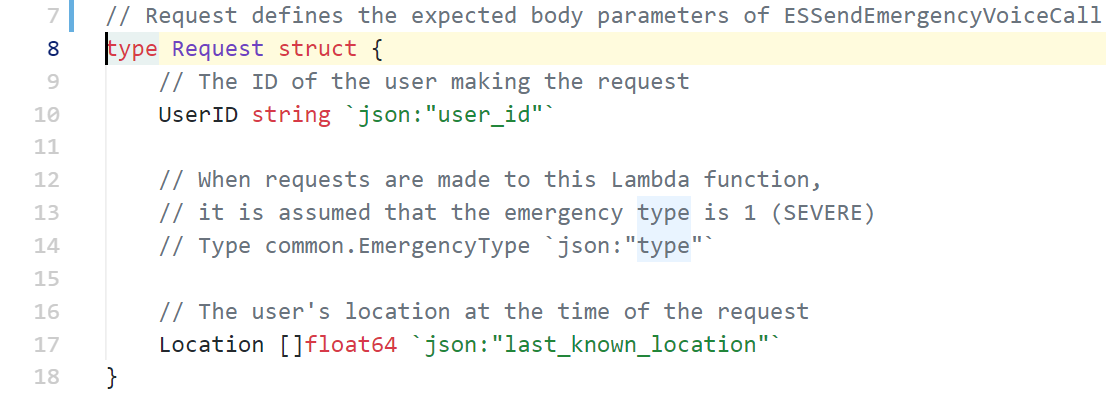
\includegraphics[scale=.6]{code-screenshots/eight.png}
  \caption{Screenshot of Request type.}
\end{figure}

\begin{figure}[H]
  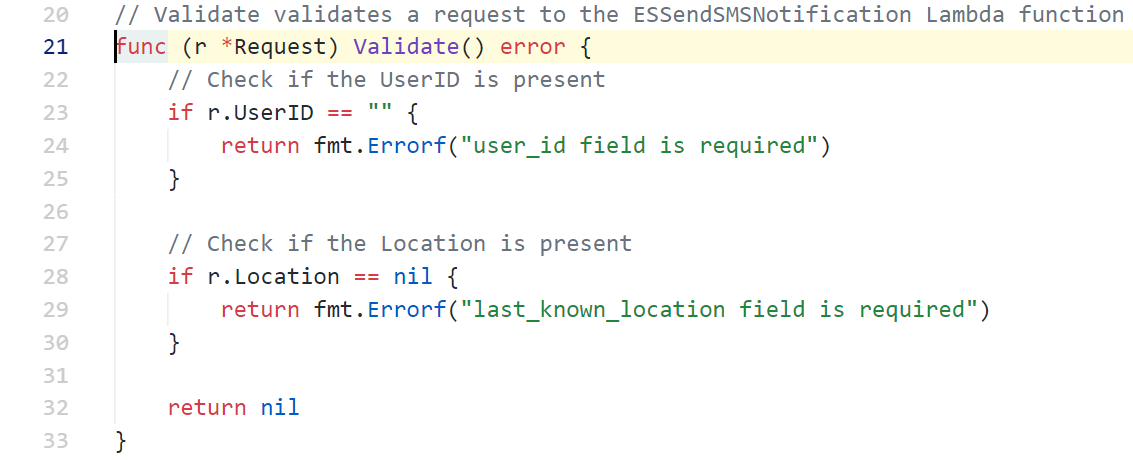
\includegraphics[scale=.6]{code-screenshots/nine.png}
  \caption{Screenshot of Validate, pointer-receiver method bound to the Request type.}
\end{figure}

\par ~ Now that the request is validated, we can continue the function execution, the flow is as follows, annotated with code line numbers present in the next six figures, and an additional two.
\begin{figure}[H]
  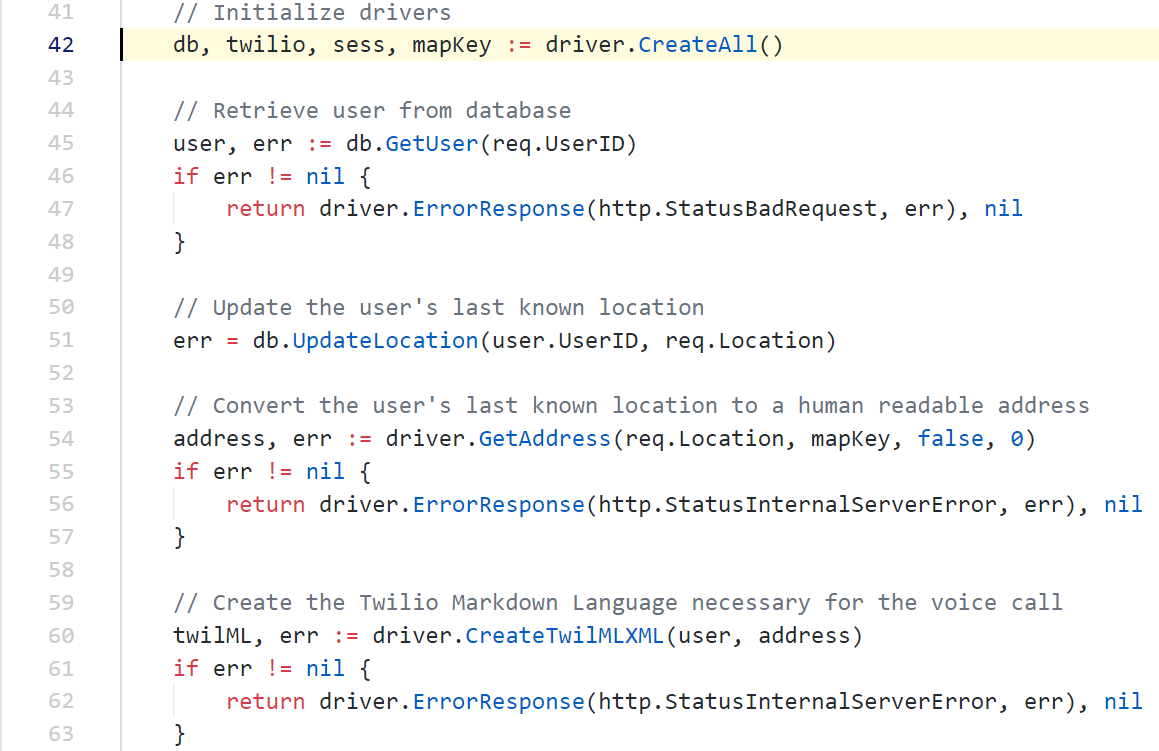
\includegraphics[scale=.6]{code-screenshots/handler-42-63.png}
  \caption{Screenshot of lines 42 through 63 of \texttt{func Handler}}\label{fig:hm}
\end{figure}

\begin{figure}[H]
  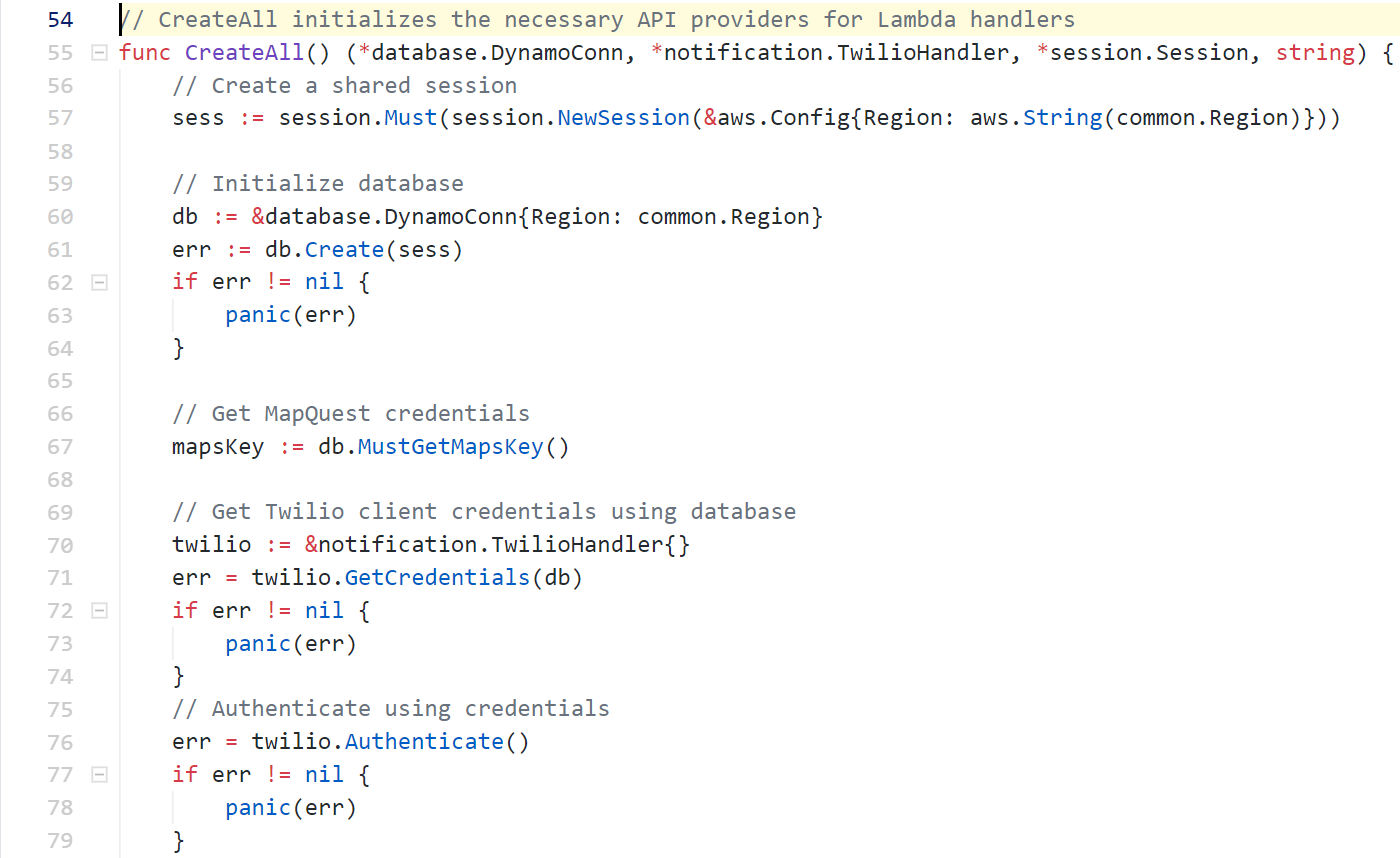
\includegraphics[scale=.6]{code-screenshots/create-all.png}
  \caption{Screenshot of \texttt{func CreateAll} within \texttt{package driver}}\label{fig:ca}
\end{figure}

\begin{figure}[H]
  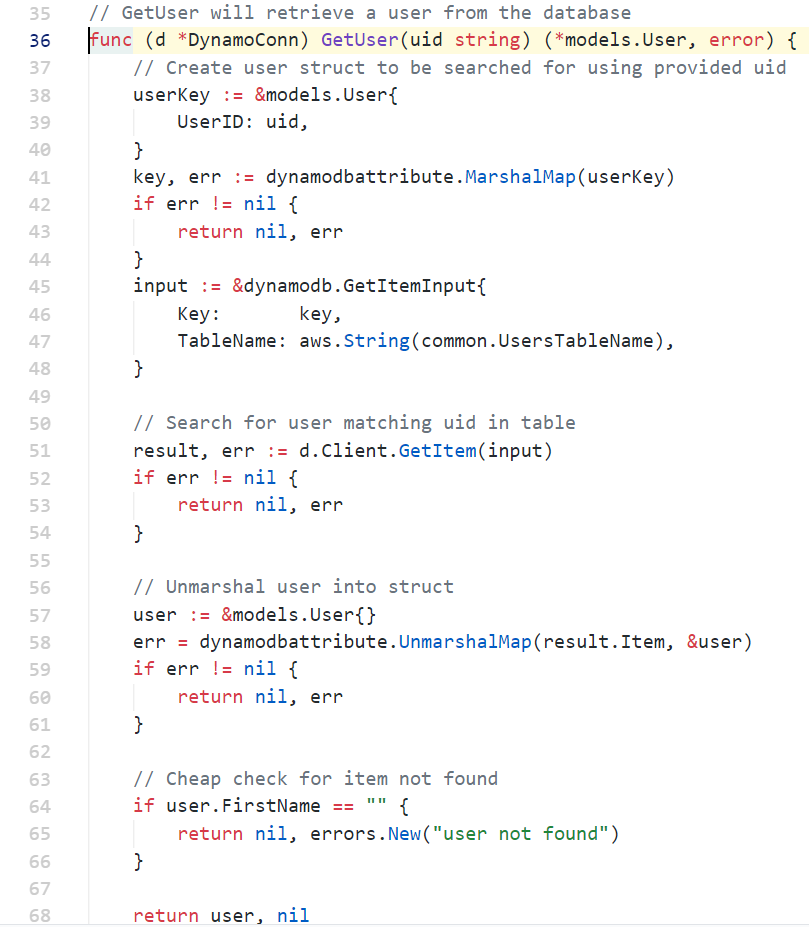
\includegraphics[scale=.6]{code-screenshots/get-user.png}
  \caption{Screenshot of \texttt{func GetUser} within \texttt{package database}}\label{fig:gu}
\end{figure}

\begin{figure}[H]
  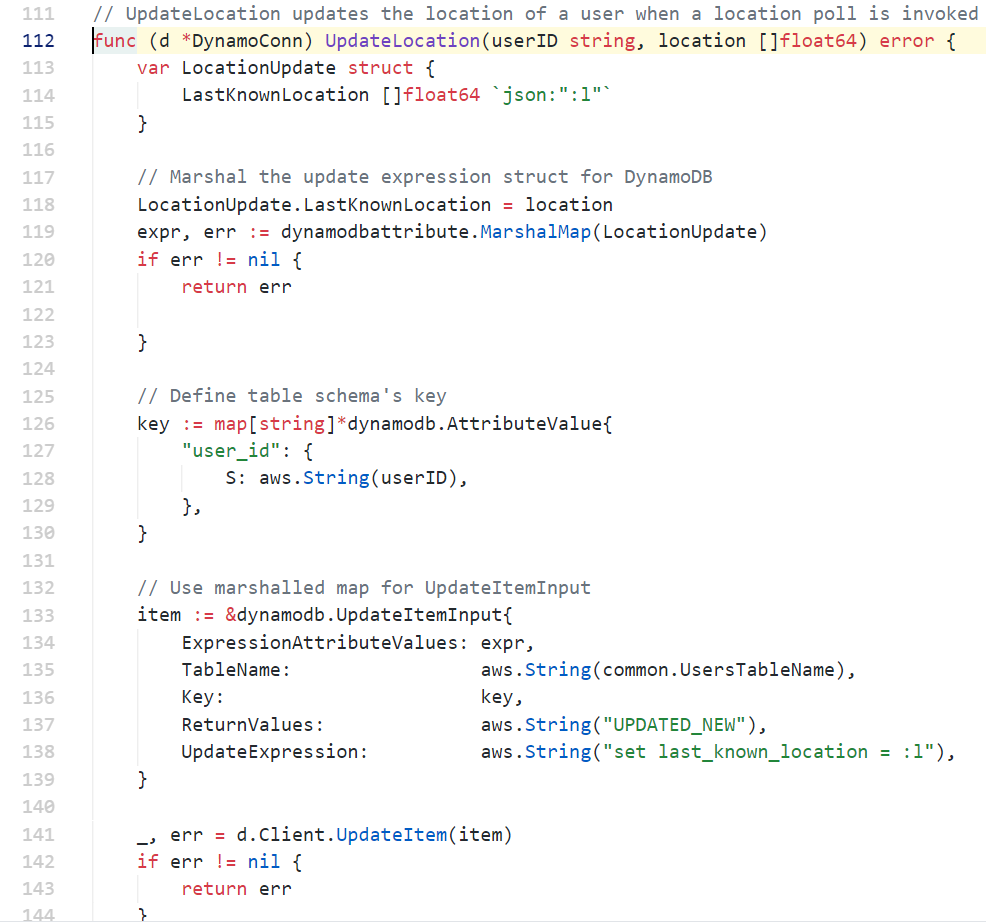
\includegraphics[scale=.6]{code-screenshots/update-location.png}
  \caption{Screenshot of \texttt{func UpdateLocation} within \texttt{package database}}\label{fig:ul}
\end{figure}

\begin{figure}[H]
  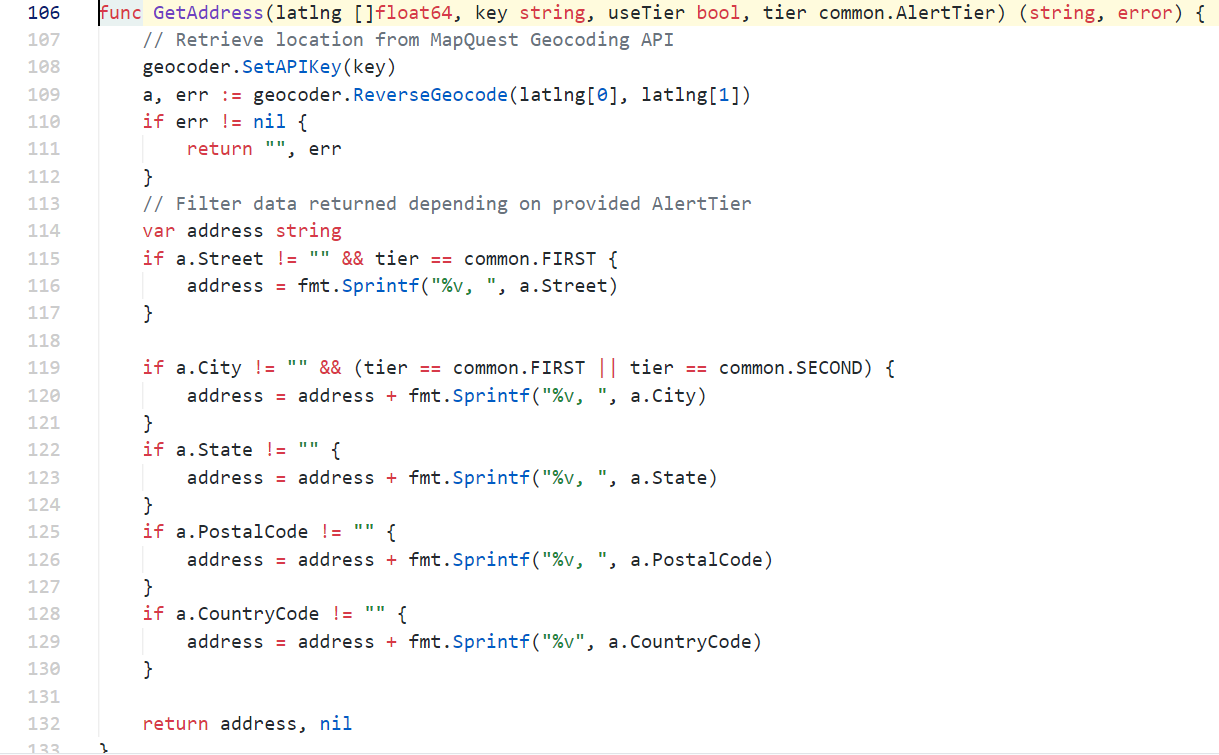
\includegraphics[scale=.6]{code-screenshots/get-address.png}
  \caption{Screenshot of \texttt{func GetAddress} within \texttt{package driver}}\label{fig:ga}
\end{figure}

\begin{figure}[H]
  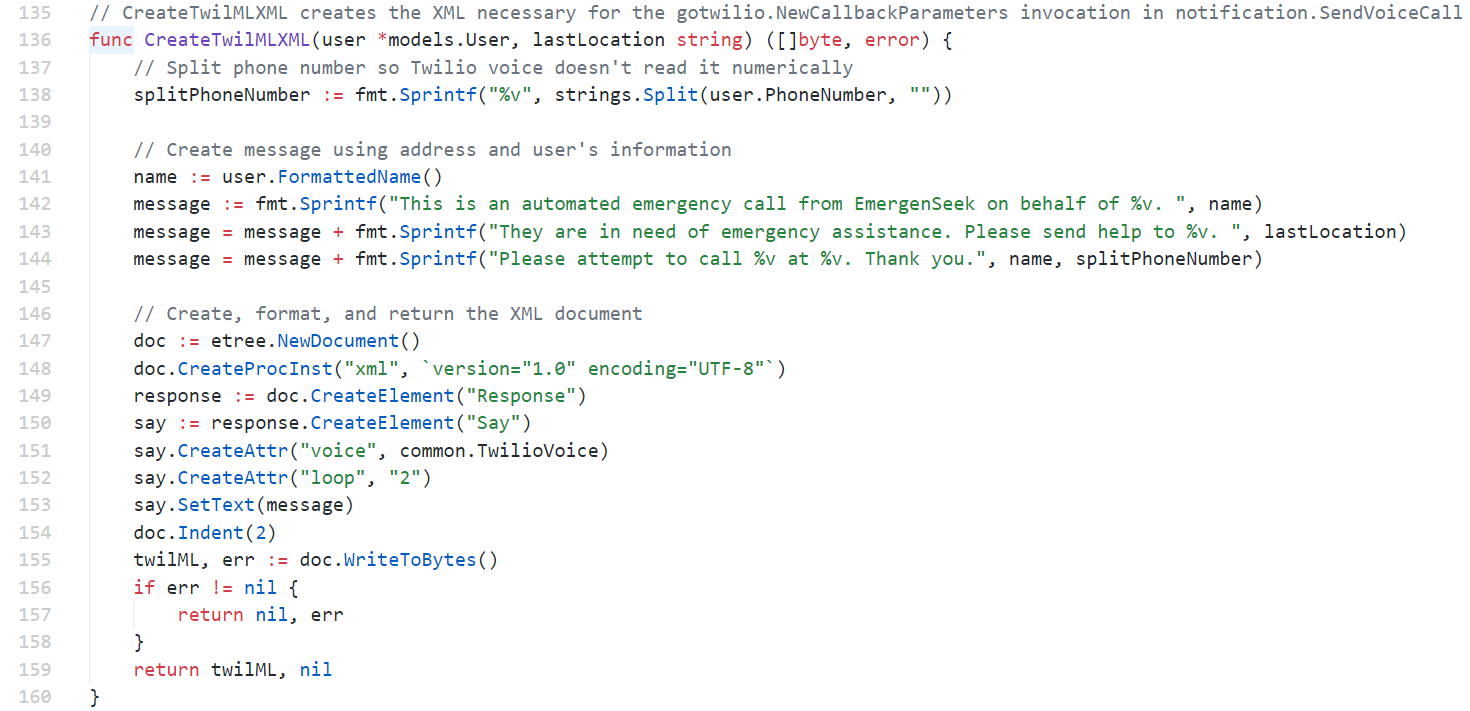
\includegraphics[scale=.6]{code-screenshots/create-twilml.png}
  \caption{Screenshot of \texttt{func CreateTwilMLXML} within \texttt{package driver}}\label{fig:ct}
\end{figure}

\par ~ First, Figure~\ref{fig:hm} line 42, we call CreateAll (Figure~\ref{fig:ca}) in the driver package. This will return 4 items, an instance of our database, a connection to our Twilio functions within the notification package, an AWS session that can be used to authenticate with different services, and mapKey used for making requests to MapQuest. Then, Figure~\ref{fig:hm} line 45, we call GetUser (Figure~\ref{fig:gu}) and return an error if the user does not exist or the request to DynamoDB fails. Continuing, Figure~\ref{fig:hm} line 51 we attempt to update the user's location by calling UpdateLocation (Figure~\ref{fig:ul}), but do not terminate the flow of the program if an error occurs, because this is a secondary functionality of the function. We try to update the user's location as they interact with various API endpoints, but cannot always guarantee the most update to date location.

\par ~ Then, Figure~\ref{fig:hm} line 54 we call GetAddress (Figure~\ref{fig:ga}) to translate the user's current location into a human readable street, city, country code and zipcode, this utilizes the MapQuest API. The last two parameters, false and 0, are workarounds for controlling whether or not we should consider alert tier, because this function is called using other Lambda functions which have this requirement. After, Figure~\ref{fig:hm} line 60, we create a TwilML (Twilio Markup Language) definition that will be passed to Twilio by calling CreateTwilMLXML (Figure~\ref{fig:ct}). This is how Twilio's voice service is programmed by developers. The language is an XML document, that contains some derectives for defining what voice will be used, how many times the content will be said, what content will be said. 

\begin{figure}[H]
  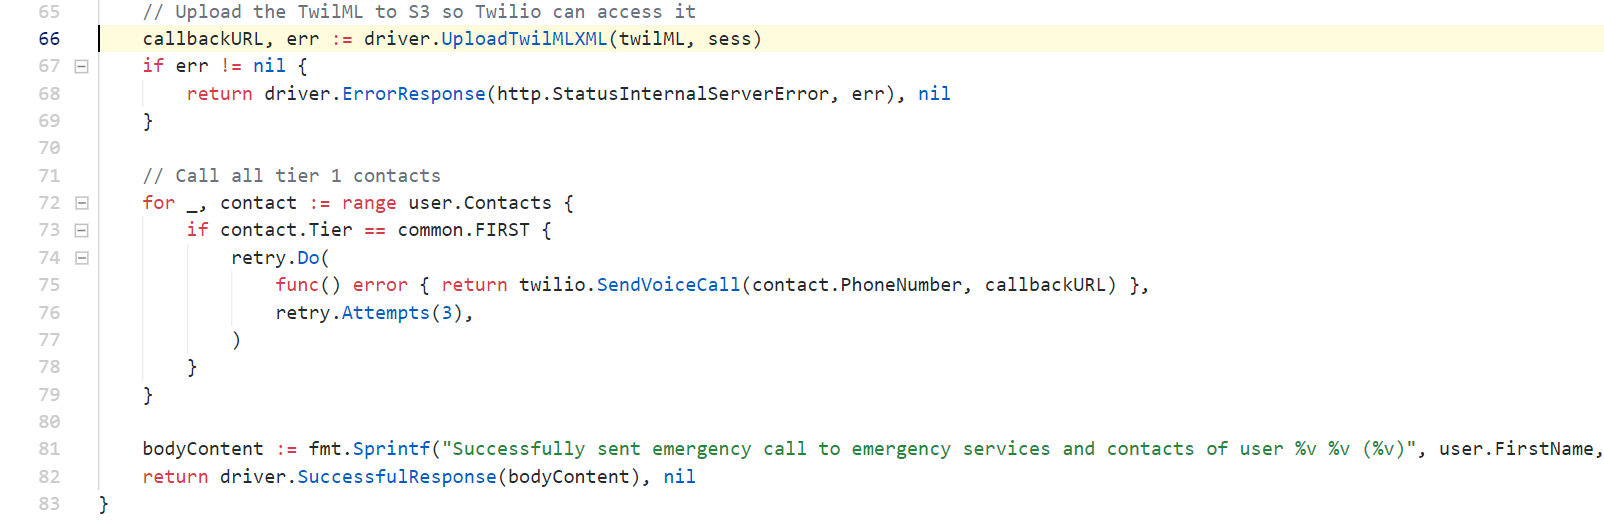
\includegraphics[scale=.6]{code-screenshots/handler-66-82.PNG}
  \caption{Screenshot of lines 66 through 82 of \texttt{func Handler}}\label{fig:hmtwo}
\end{figure}

\begin{figure}[H]
  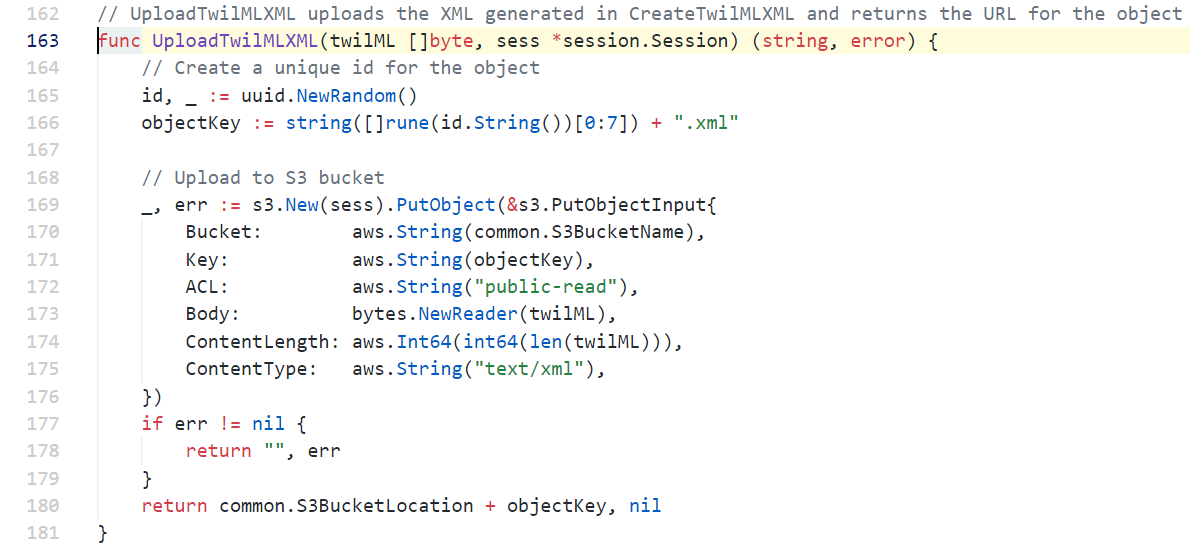
\includegraphics[scale=.7]{code-screenshots/upload-twilml.PNG}
  \caption{Screenshot of \texttt{func UploadTwilMlXML} within \texttt{package driver}}\label{fig:ut}
\end{figure}

\par ~ To make this document accessible to Twilio's API, we upload it to Amazon's Simple Storage Service (S3) at Figure~\ref{fig:hmtwo} line 66 by calling UploadTwilMlXML (Figure~\ref{fig:ut}). At the end of \texttt{func Handler} in Figure~\ref{fig:hmtwo}, lines 81 and 82 entail responding to the requesting client with a HTTP 200 OK response and a generic, identifiable message.

\subsection{Informal Testing}
\par ~ Now that we have written the Lambda function, we can informally test it. To do this we use will use the Serverless Application Model command-line interface (SAM CLI) \cite{three}. Installation and setup details are available in the README.md file of our backend repository. The SAM CLI allows us to test our application in a Docker container, similar to the environment provided by AWS, in the cloud. Instead of deploying the application and later discovering that we have issues, we can catch those issues much quicker by doing the testing and debugging in our local environment. Doing this is as follows.

\begin{enumerate}
	\item[1.] Define a SAM template.yml definition. This YAML definition will define our Lambda function and API Gateway Endpoint.
	\item[2.] Start Docker
	\item[3.] Run \texttt{make sam} to run a series of commands that build, package, and start the local API
	\item[4.] Run \texttt{make test} to test the endpoint using the sample request defined in \texttt{event.json}
\end{enumerate}

\begin{figure}[H]
  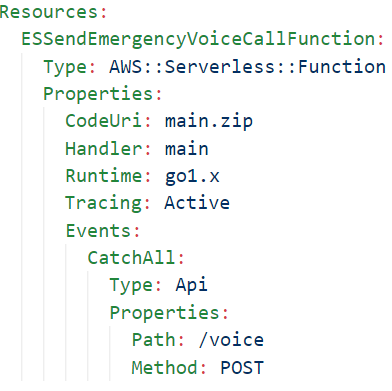
\includegraphics[scale=.7]{code-screenshots/local-template.png}
  \caption{Screenshot of the local template.yml used for SAM.}
\end{figure}
\begin{figure}[H]
  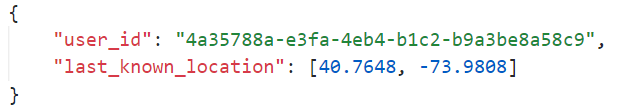
\includegraphics[scale=.7]{code-screenshots/event.PNG}
  \caption{Screenshot of the event.json used for locally testing this function.}
\end{figure}
\begin{figure}[H]
  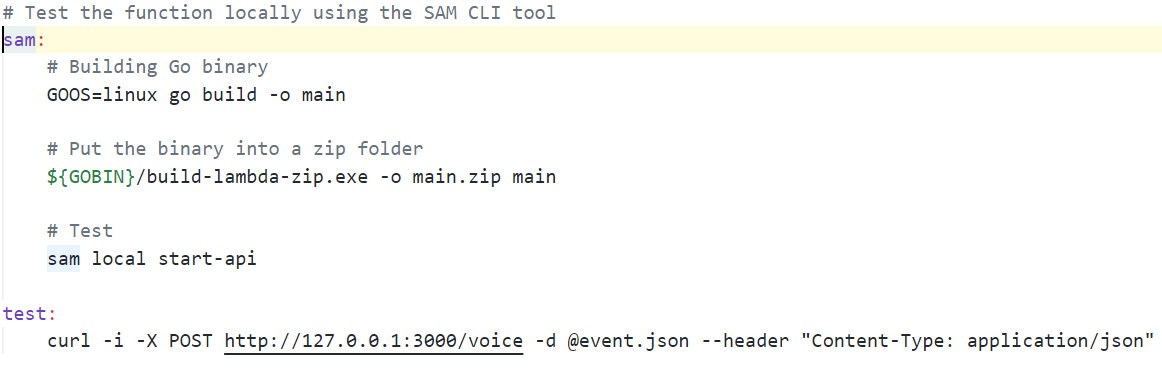
\includegraphics[scale=.7]{code-screenshots/makefile.PNG}
  \caption{Screenshot of the Makefile rules used to make testing more convenient.}
\end{figure}

\subsection{Formal Testing}
\par ~ Next, now that we're confident, that our function behaves as expected we can write formal unit tests for it. These tests are defined in a functions main\_test.go file. The file defines one function for unit testing the handler, and a testing object. This testing object is apart of the Go standard library and provides many useful tools for writing tests. The tests for our application, although not all have unit tests, follow the table-driven testing (TDD) pattern. Tests are given some expected paramters and are looped over to cover different edge cases. For this test, we only have one test in the table. This test also uses a pre-defined user id, located in a DynamoDB table.
\begin{figure}[H]
  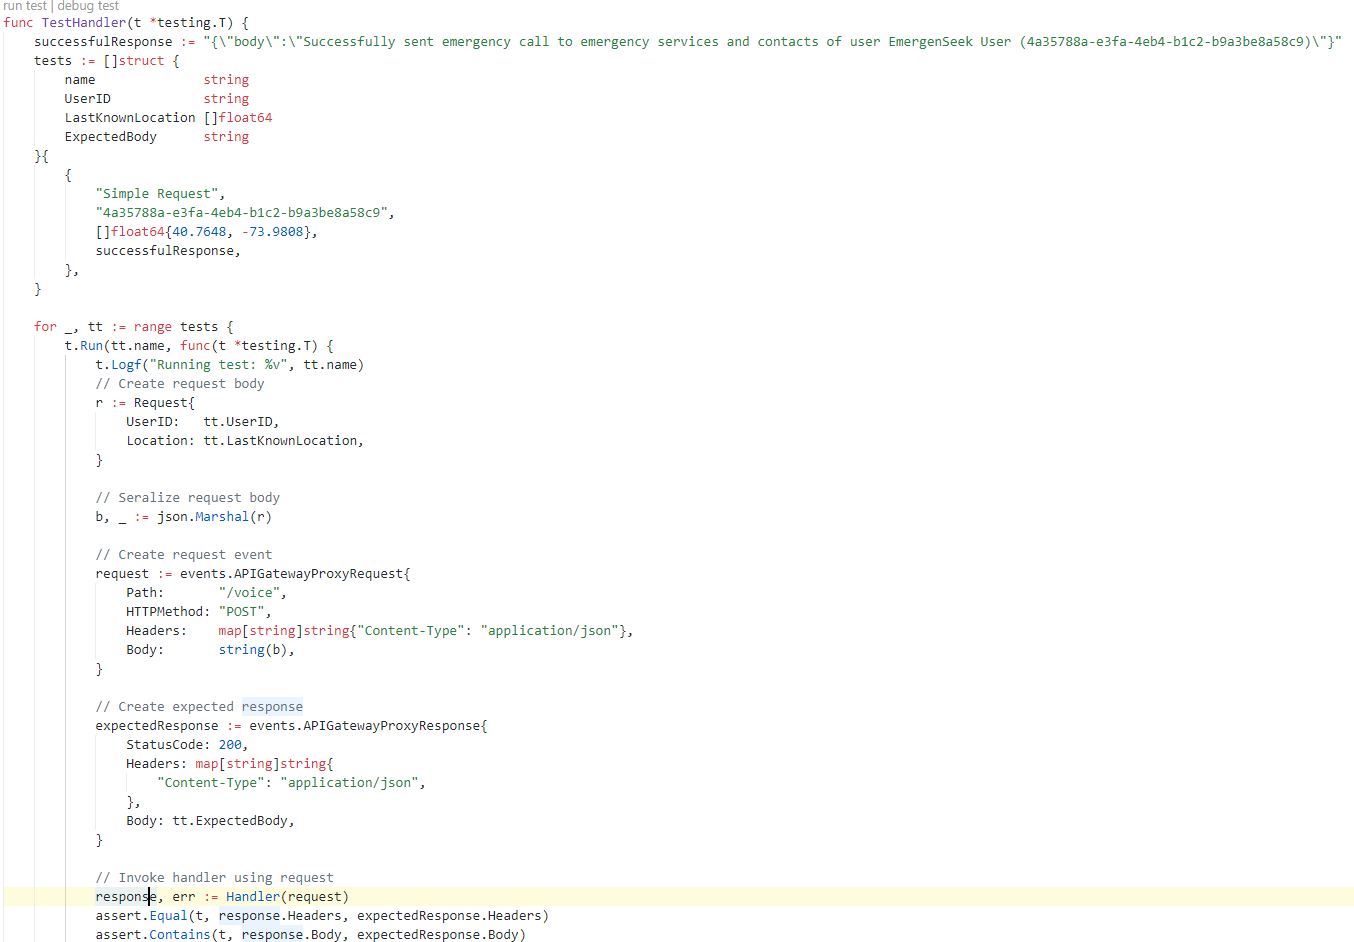
\includegraphics[scale=.7]{code-screenshots/main-test.PNG}
  \caption{Screenshot of the test function located in main\_test.go for testing \texttt{func Handler} of ESSendEmergencyVoiceCall.}
\end{figure}

\subsection{Deployment}
\par ~ Continuing, now that we have defined a formal test, we can proceed to pushing our code to the master branch of our repository and begin the deployment. To do this, we update our buildspec.yml and template.yml in the root of the repository. Changes to the template.yml are similar to the initial creation of the file we made for local SAM CLI for testing. 
\begin{enumerate}
	\item[1.] Update buildspec pre\_build stage with:
	\begin{center}
		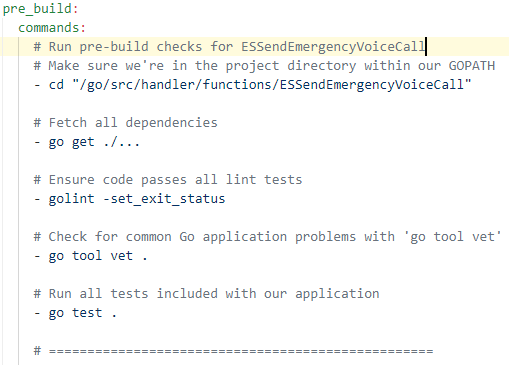
\includegraphics[scale=1]{code-screenshots/pre-build.PNG}
	\end{center}
	\item[2.] Update buildspec build stage with :
	\begin{center}
		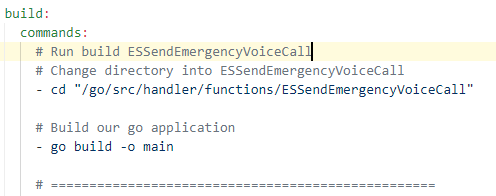
\includegraphics[scale=1]{code-screenshots/build.PNG}
	\end{center}
	\item[3.] Add new resource and matching route/request method to template.yml:
	\begin{center}
		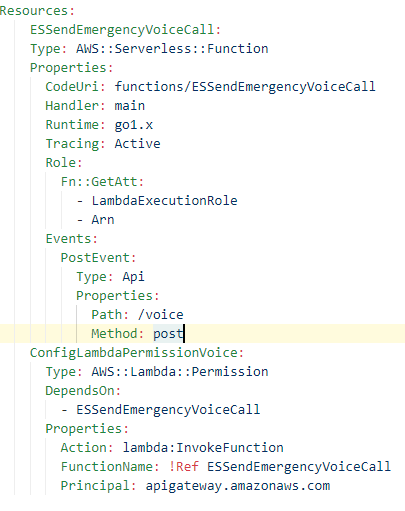
\includegraphics[scale=1]{code-screenshots/deploy-template.PNG}
	\end{center}
\end{enumerate}

\par ~ After adding, committing,and pushing to the master branch of our GitHub repository, AWS CodeStar will take over and handle our continuous integration and continuous deployment by using the definitions in the buildspec.yml and template.yml.

\begin{figure}[H]
\begin{center}
  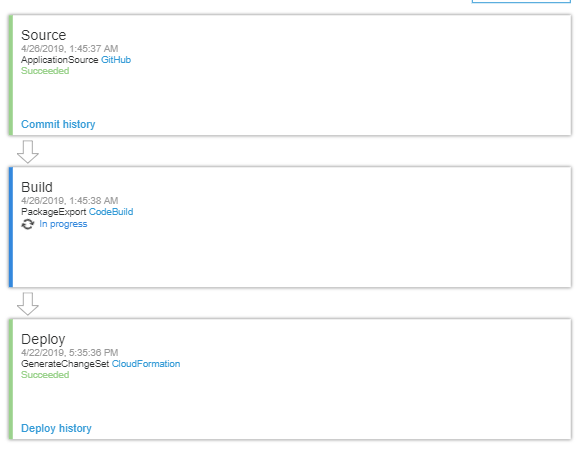
\includegraphics[scale=.7]{build-in-progress.PNG}
  \caption{AWS CodeStar screenshot of a build in progress, after a Git Push to our code repository.}
\end{center}
\end{figure}

\begin{figure}[H]
\begin{center}
  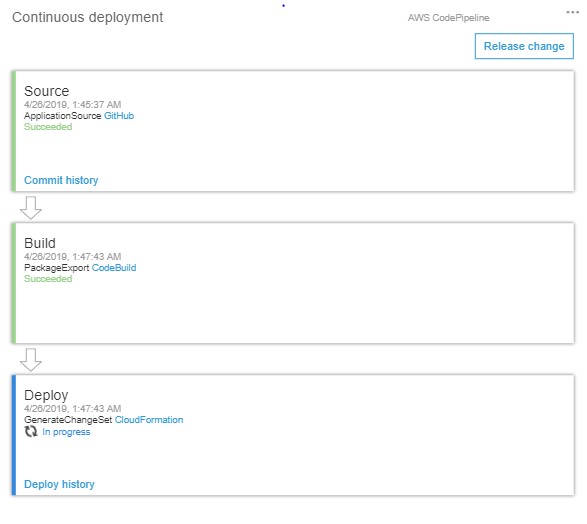
\includegraphics[scale=.7]{deploy-in-progress.PNG}
  \caption{AWS CodeStar screenshot of a deploy in progress, after a successful build.}
\end{center}
\end{figure}

\begin{figure}[H]
\begin{center}
  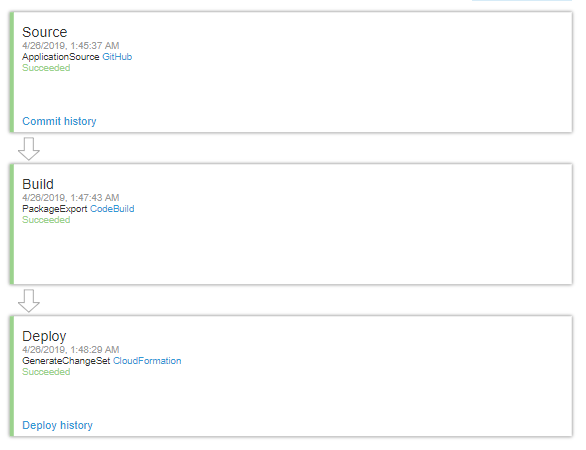
\includegraphics[scale=.7]{successful-deploy.PNG}
  \caption{AWS CodeStar screenshot a successful CI/CD pipeline; deploy complete.}
\end{center}
\end{figure}

\subsection{Integration}
\par ~ Next, now that the function is deployed, we can begin connecting the frontend. First, we'll need the endpoint at which the function lives. To find this, we can navigate to API Gateway in the AWS console.
\begin{figure}[H]
\begin{center}
  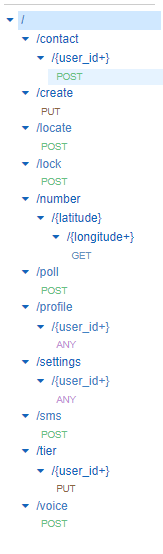
\includegraphics[scale=1]{code-screenshots/all-endpoints.PNG}
  \caption{AWS API Gateway screenshot of all endpoints we have available for access.}
\end{center}
\end{figure}

\begin{figure}[H]
\begin{center}
  
\includegraphics[scale=1]{code-screenshots/invoke-url.PNG}
  \caption{AWS API Gateway screenshot of our production stage, Invoke URL}
\end{center}
\end{figure}

\par ~ First we create the feature view. This is defined in sos.dart within the screens folder, encapsulated in the lib folder. The feature view is made up of several widgets, each acting as a container, or higher-level parent to perform some function. The SOSPage encapsulates the SOSButton as its parent. The SOSButton encapsulates the ProgressRing StatefulWidget which will call the activateSOS method. The ProgressRing has a method called showConfirmation which will allow the user to select their emergency tier or cancel.

\begin{figure}[H]
\begin{center}
  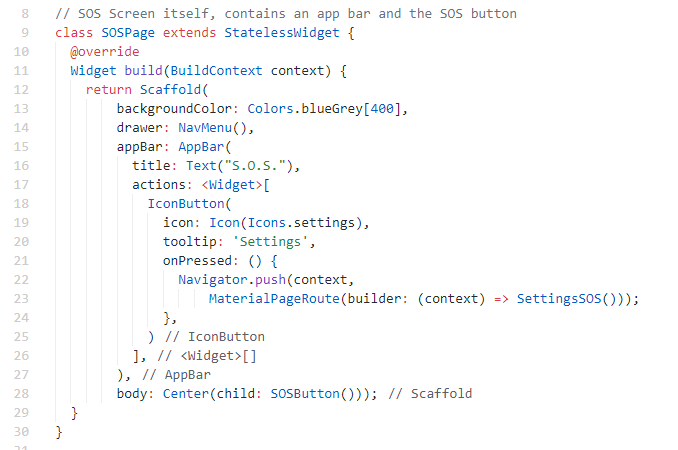
\includegraphics[scale=1]{code-screenshots/sospage.PNG}
  \caption{Screenshot of the SOSPage widget's Dart class}
\end{center}
\end{figure}
\begin{figure}[H]
\begin{center}
  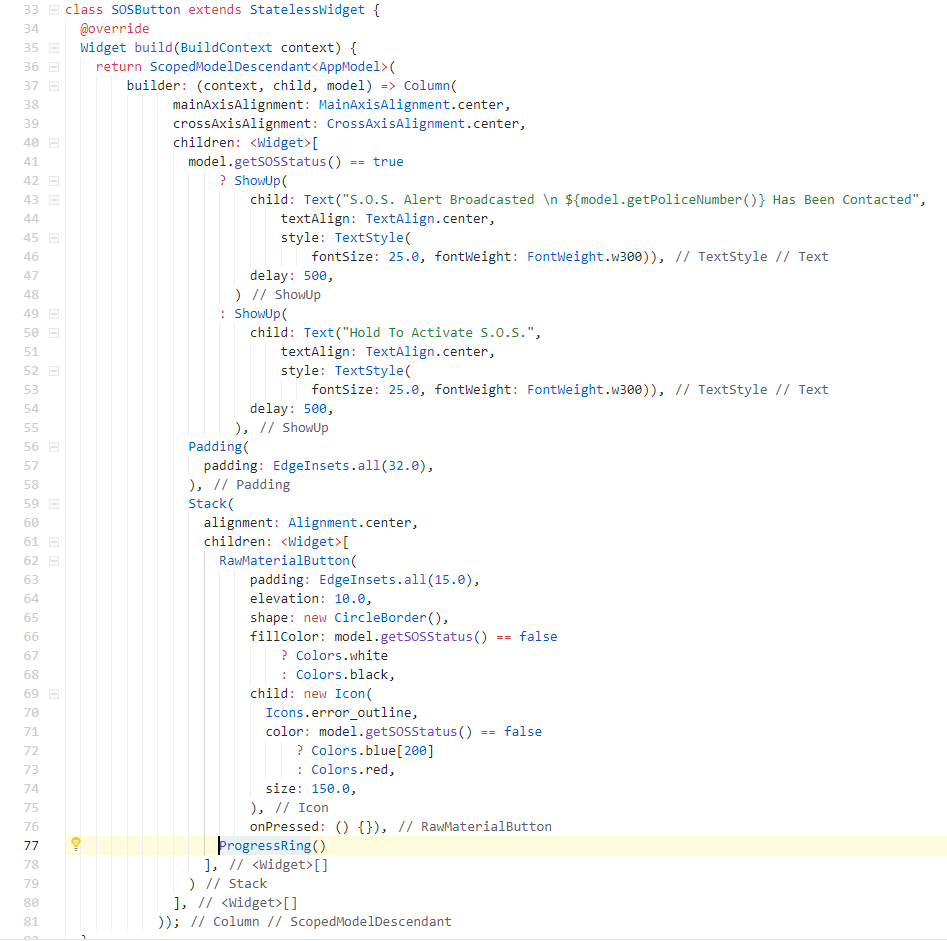
\includegraphics[scale=1]{code-screenshots/sosbutton.PNG}
  \caption{Screenshot of the SOSButton widget's Dart class}
\end{center}
\end{figure}
\begin{figure}[H]
\begin{center}
  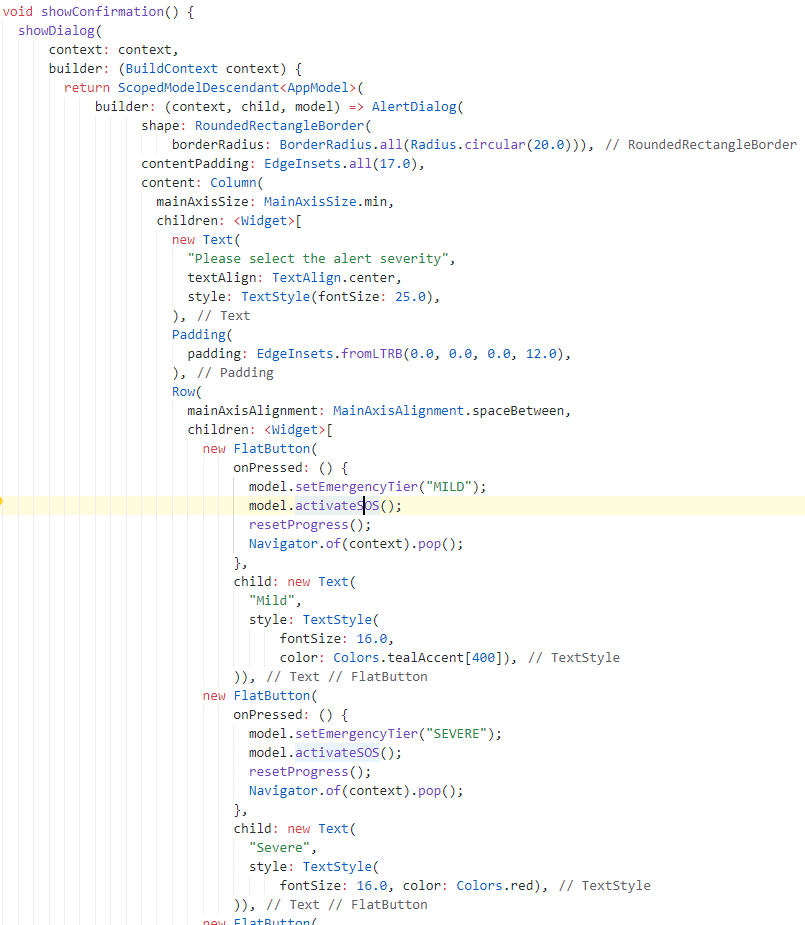
\includegraphics[scale=1]{code-screenshots/show-confirmation.PNG}
  \caption{Screenshot of the showConfirmation method of ProgressRing StatefulWidget.}
\end{center}
\end{figure}

\par ~ The activateSOS method is the beginning of the model implementation. The model will encapsulate calls to a service method that will invoke the Lambda function directly
\begin{figure}[H]
\begin{center}
  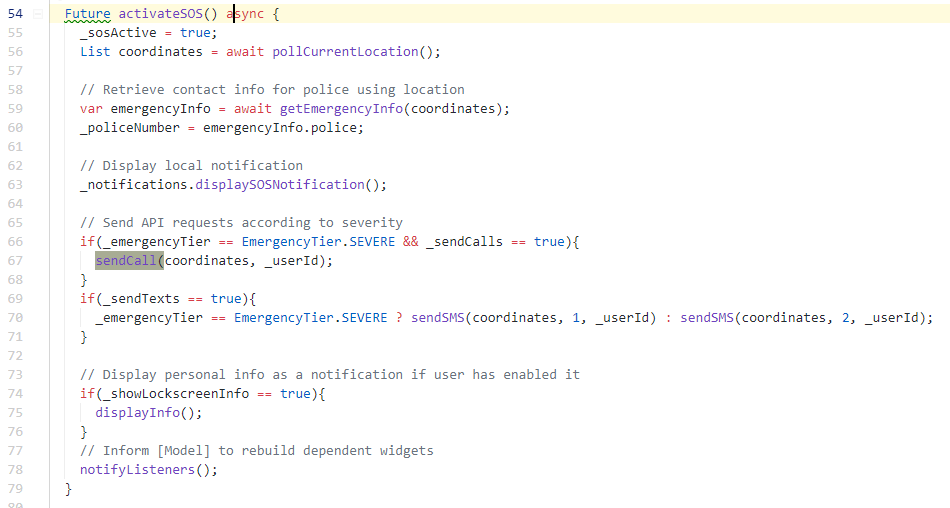
\includegraphics[scale=1]{code-screenshots/activate-sos.PNG}
  \caption{Screenshot of the activeateSOS method within the SOSModel class, a scoped model.}
\end{center}
\end{figure}


\par ~ The method which invokes the Lambda function directly is implemented as callSOS. Note that the URL and path is the same as our Invoke URL and the path the we defined for the Lambda function. Also note the \texttt{http.post} call on the url. This is important because we defined that the application should only accept POST requests.
\begin{figure}[H]
\begin{center}
  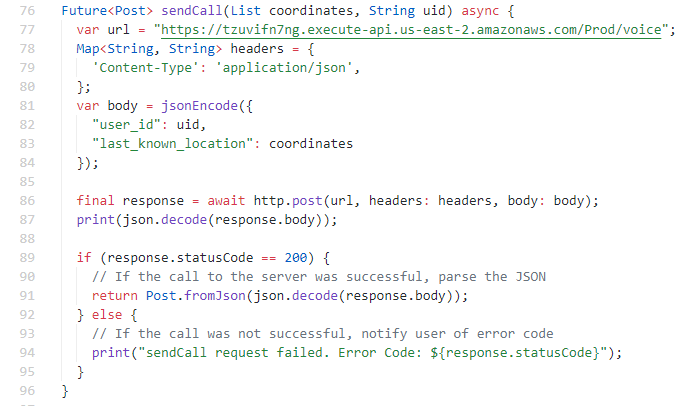
\includegraphics[scale=1]{code-screenshots/send-call.PNG}
  \caption{sendCall service function within the api.dart file of the services package}
\end{center}
\end{figure}




\section{Conclusion}
\subsection{Implementation Challenges}
\subsubsection{Lambda Maximum Compute Time Limitation}
\par ~ Throughout the development of the project, the only limitation that we have found as a result of using Lambda comes from the maximum compute time. Because Lambda instances are derived on a per-request basis (customers are charged for the amount of time their functions are running), there is a maximum cap of 15-minutes at which a single Lambda function can run for a single request. Because of this we have not been able to implement ESPollLoop, which will give our application the ability to send notifications on a periodic, repeating basis.

\subsubsection{Identity Access and Management}
\par ~ Similarly to our partial demo and implementation, one of the largest implementation issues we have had thus far is the integration of AWS CloudFormation for automatically provisioning the resources necessary for creating each Lambda function and their respective API Gateway route. Overall, assigning the correct permissions for the service workers responsible for creating these resources is the biggest issue. We currently still need to correct this issue.

\subsection{Group Member Contributions}
\par ~ 


\section{Glossary}
\begin{enumerate}
	\item[$\bullet$] Cross-platform application - software which has a single implementation, but may be executed on different distributions. (i.e. one code base, running on many different operating systems or processor architectures.)
	\item[$\bullet$] Serverless application repository - single responsibility application definitions which act as independent entities. The application repository as a whole defines the API for our mobile application. (i.e. each serverless application is a Lambda function, and the lambda function is responsible for a system feature.)
	\item[$\bullet$] Application Programming Interface (API) - Definitions and communication protocols used for building the structure of software.
	\item[$\bullet$] HyperText Transfer Protocol (HTTP) - An application protocol used heavily for websites and services throughout the Internet.
	\item[$\bullet$] REpresentational State Transfer (REST) - A architectural style for APIs that define some specifications for creating web-based services.
\end{enumerate}

\begin{thebibliography}{9}
\bibitem{one}
scoped\_model 1.0.1 | Flutter Package --- \url{https://pub.dartlang.org/packages/scoped_model}
\bibitem{two} 
		Mattihas Jung, Sascha Möllering, Peter Dalbhanjan, Peter Chapman, Christoph Kassen \\
		\textit{Microservices on AWS; AWS Whitepaper}. \\
		\texttt{\url{https://docs.aws.amazon.com/aws-technical-content/latest/microservices-on-aws/microservices-on-aws.pdf}}
\bibitem{three}
What is the AWS Serverless Application Model (AWS SAM)? --- \url{https://docs.aws.amazon.com/serverless-application-model/latest/developerguide/what-is-sam.html}
\end{thebibliography}

% Appendix of figures
\begin{appendix}
	\listoffigures
\end{appendix}

\end{document}

